% \begin{abstract}
% We replicated the reinforcement-learning ramp-metering method proposed by Yang et al.~(2025) in the paper ``Reinforcement Learning–Based Ramp Metering Strategy Considering Queue Management'', focusing on its action replacement module for preventing ramp queue spillback during training. Because the original code, SUMO networks, demand data, and training configuration were unavailable, we reconstructed the single-ramp and multi-ramp environments and implemented the controllers and training pipeline from the published description. The safety mechanism was partially replicated. In the multi-ramp experiment, action replacement reduced spillback events without degrading the converged policy, and its use declined to approximately 1\% of actions. The single-ramp experiment showed weaker agreement, and the reported absolute travel-time improvements could not be reproduced. These differences were strongly affected by undocumented demand profiles, network parameters, and training choices. The results support the qualitative value of action replacement but do not independently confirm the original study's quantitative performance claims.
% \end{abstract}

\section*{Replication Summary}

\subsubsection{Scope of Replication}

We replicated the main results and claims of Yang et al.~\cite{Yang2025Reinforcement}. The original study ``Reinforcement Learning–Based Ramp Metering Strategy Considering Queue Management'' proposes an action replacement module for reinforcement-learning-based ramp metering. A store-and-forward model estimates the minimum metering rate required to avoid queue spillback; actions below this lower bound are replaced and penalised. The claimed benefit is safer training without reduced convergence speed or final control performance. We evaluated this claim in independently reconstructed single-ramp and multi-ramp SUMO environments and compared the proposed controller with no control, PI-ALINEA \cite{wang2014local}, HERO \cite{Papamichail2010HERO}, and an unconstrained RL baseline.

\subsubsection{Methodology}

No original code, SUMO networks, demand data, or complete training configuration were available. We reconstructed the networks from published figures and satellite imagery and implemented the simulation interface, benchmark controllers, action replacement module, and PPO training pipeline in Python. The single-ramp experiments use the demand profile reported in the original paper. The missing multi-ramp demand was estimated by matching the original no-control speed heatmap. Controller performance was evaluated across ten random seeds.


\subsubsection{Results}

The results provide partial support for the proposed safety mechanism but do not reproduce the original quantitative performance claims. In the multi-ramp safety experiment, action replacement reduced late spillback failures, preserved performance relative to the constrained baseline, and declined to approximately 1\% of actions. In the single-ramp experiment, training was smoother, but approximately 7\% of actions were still replaced at convergence. The reported TTS reductions and several traffic patterns were not reproduced. These differences are strongly affected by unavailable demand data, network parameters, and training settings.


\subsubsection{What was easy}

The high-level reinforcement-learning pipeline and benchmark-controller interfaces were straightforward to implement.


\subsubsection{What was difficult}

The main difficulty was reconstructing the SUMO environments. On-ramp merging behaviour, network capacity, multi-ramp demand, queue storage, and several training parameters were not specified in sufficient detail. Small changes to these choices produced substantial differences in congestion and controller behaviour.


\subsubsection{Communication with the authors}

We attempted to contact the authors multiple times but did not receive a response. No source code, detailed algorithmic parameters, or supplementary materials were available beyond those provided in the published manuscript.

% \newpage

% Introduction
\section{Introduction}

Ramp metering controls the rate at which vehicles enter a motorway from an on-ramp, to mitigate congestion on highways. An effective controller must improve mainline traffic flow without allowing the ramp queue to spill back onto adjacent roads \cite{Trubia2021RampMetering}. Reinforcement-learning controllers can optimise this trade-off, but exploration during training may produce unsafe actions \cite{han2023leveraging}.

Yang et al.~(2025)~\cite{Yang2025Reinforcement} proposed an action replacement module for reinforcement-learning-based ramp metering. The module computes a lower bound on the metering rate from a store-and-forward traffic model. Actions below this bound are replaced and penalised during training. The original study reported that this mechanism prevented queue spillback without reducing convergence speed or final control performance. It evaluated the method in single-ramp and multi-ramp SUMO simulations \cite{lopez2018microscopic}.

The original implementation, simulation networks, demand data, and complete training configuration were not publicly available. We therefore reconstructed both simulation environments from the information in the article and implemented the proposed method, benchmark controllers, and training pipeline independently. We compared the replicated results directly with the original figures and performance tables and evaluated the controllers across multiple random seeds. Our objective was to determine to which extent reported results could be replicated and whether the action replacement module provided the claimed safety benefit without compromising traffic performance. Our results partially validate the claims of the original study. While we confirmed that the action replacement module improves training safety by reducing spillback events, the exact reported quantitative performance benefits could not be reproduced due to missing simulation parameters.

\section{Summary of Original Study}

The original study proposes an action replacement module for ramp metering based on Proximal Policy Optimisation (PPO) \cite{Schulman2017PPO}. A store-and-forward model computes a lower bound on the metering rate at each control step. Any agent action below this bound is replaced, and a penalty proportional to the traffic state's proximity to spillback is applied. The module is intended to prevent spillback during training while encouraging the agent to learn safe actions.

\begin{figure}[!h]
    \centering
    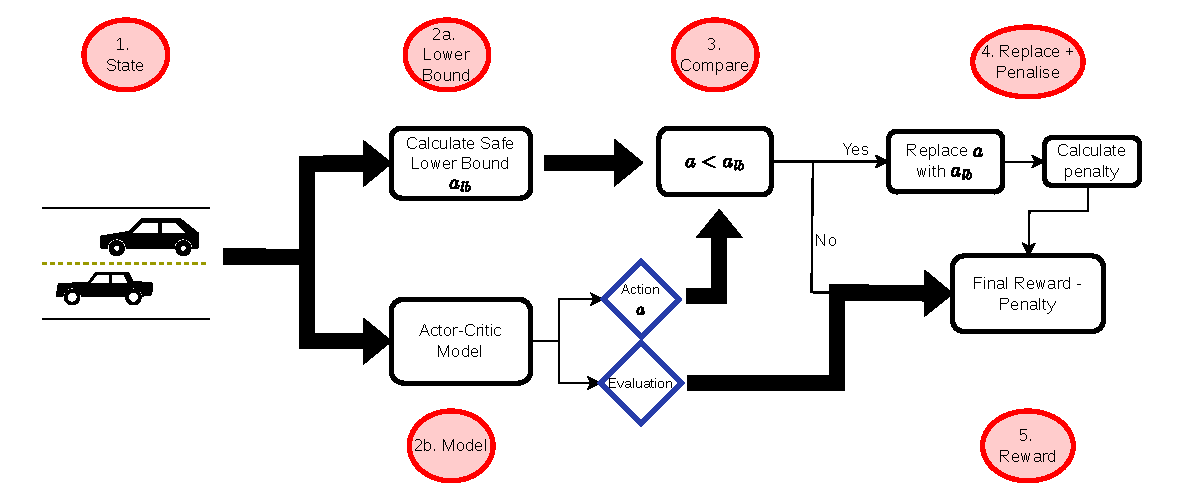
\includegraphics[width=1\linewidth]{figures/method_summary.pdf}
    \caption{Logic of the action replacement module. The proposed action is compared with a lower bound derived from the store-and-forward model. An action below the bound is replaced and a spillback penalty is subtracted from the step reward.}
    \label{fig:method_summary}
\end{figure}

The method is evaluated in both single-ramp and multi-ramp scenarios using the SUMO microscopic traffic simulator, calibrated against real-world flow data from the Nanjing Ring Freeway. In the single-ramp scenario, the proposed RL controller reduces TTS by 5.17\% over the no-control baseline and outperforms PI-ALINEA, while the action replacement module is shown to reduce the proportion of unsafe actions over the course of training from an initial rate of ~25\% to nearly zero. In the multi-ramp scenario, the RL controller achieves the lowest TTS among all tested strategies, and the action replacement module again successfully eliminates spillback events without degrading convergence speed or final performance.


\section{Implementation Details}
\label{sec:implementation_details}

Neither the SUMO network files nor the training code were made available by the authors. The simulation environment, all benchmark controllers, and the full RL training pipeline were therefore reconstructed from scratch using only the information contained in the published manuscript.

\subsubsection{Simulation Environment}

\paragraph{Single-Ramp Scenario.} The single-ramp scenario replicates the Shiyang Road on-ramp of the Nanjing Ring Expressway (32$^\circ$00'37.6''N, 118$^\circ$50'50.7''E). A corridor of approximately 1.34~km was reconstructed from Figure~4 of the original paper. The mainline has four lanes and a reported capacity of 8{,}280~veh$\cdot$h. The on-ramp has two lanes, a reported capacity of 1{,}930~veh$\cdot$h, and a reported maximum storage of $w_{\max}=42$ vehicles. Upstream virtual edges were set to 200~m for the mainline and 100~m for the on-ramp because their lengths were not reported.

\begin{figure}[!h]
    \centering
    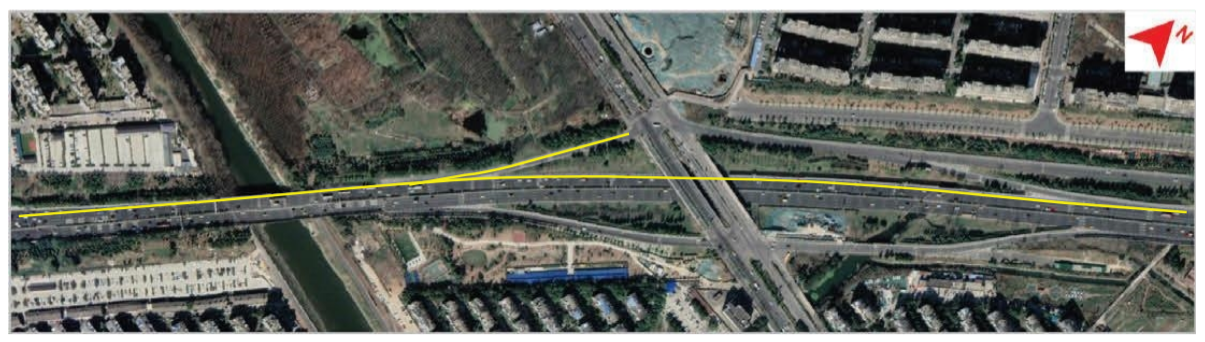
\includegraphics[width=0.9\linewidth]{figures/yang2025_fig4.png}\\[0.5em]
    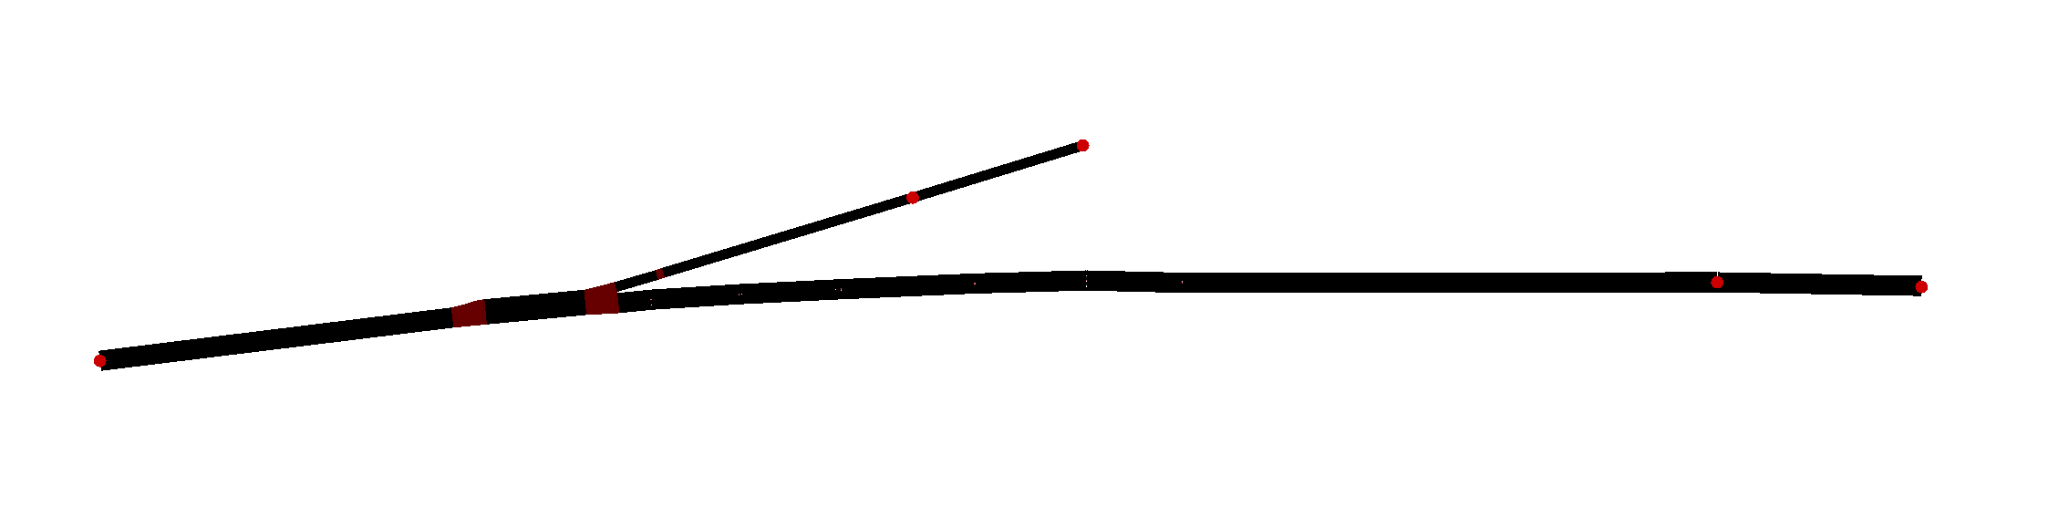
\includegraphics[width=0.9\linewidth]{figures/yang2025_fig4_rep.png}
    \caption{Satellite map of the single-ramp test corridor (Shiyang Road on the Nanjing Ring Expressway). Top: original from~\cite{Yang2025Reinforcement}, Figure~4. Bottom: reconstructed test segment used in the replication.}
    \label{fig:single_ramp_map}
\end{figure}

Each simulation step represents one second of real time. Each control step spans 15 simulation steps (15~s). An episode runs for a maximum of 240 control steps (3{,}600~s total). An episode is terminated early if the ramp queue exceeds 90\% of maximum capacity, i.e.\ $w(k) > 0.9 \times 42 = 37.8$~vehicles, consistent with the criterion stated in the original paper.

The maximum storage of 42 vehicles was confirmed by holding the ramp signal at red until the queue reached steady state. The mainline capacity could not be verified because the original study does not define how it was measured. The reconstructed ramp also had a substantially lower empirical capacity than the reported 1{,}930~veh$\cdot$h. This difference affects the action replacement module because the reported capacity is used in its lower-bound calculation.

Traffic demand inputs were reconstructed from the original paper (Figure~\ref{fig:single_ramp_demand}). The paper reports a stepwise profile in which the mainline demand rises from 7{,}400~veh$\cdot$h to 7{,}900~veh$\cdot$h at $t = 600$~s and remains constant until $t = 3{,}300$~s before falling to 4{,}000~veh$\cdot$h; the ramp demand rises from 600~veh$\cdot$h to 1{,}300~veh$\cdot$h at $t = 600$~s and falls to 500~veh$\cdot$h at $t = 3{,}600$~s.

\begin{figure}[!h]
    \centering
    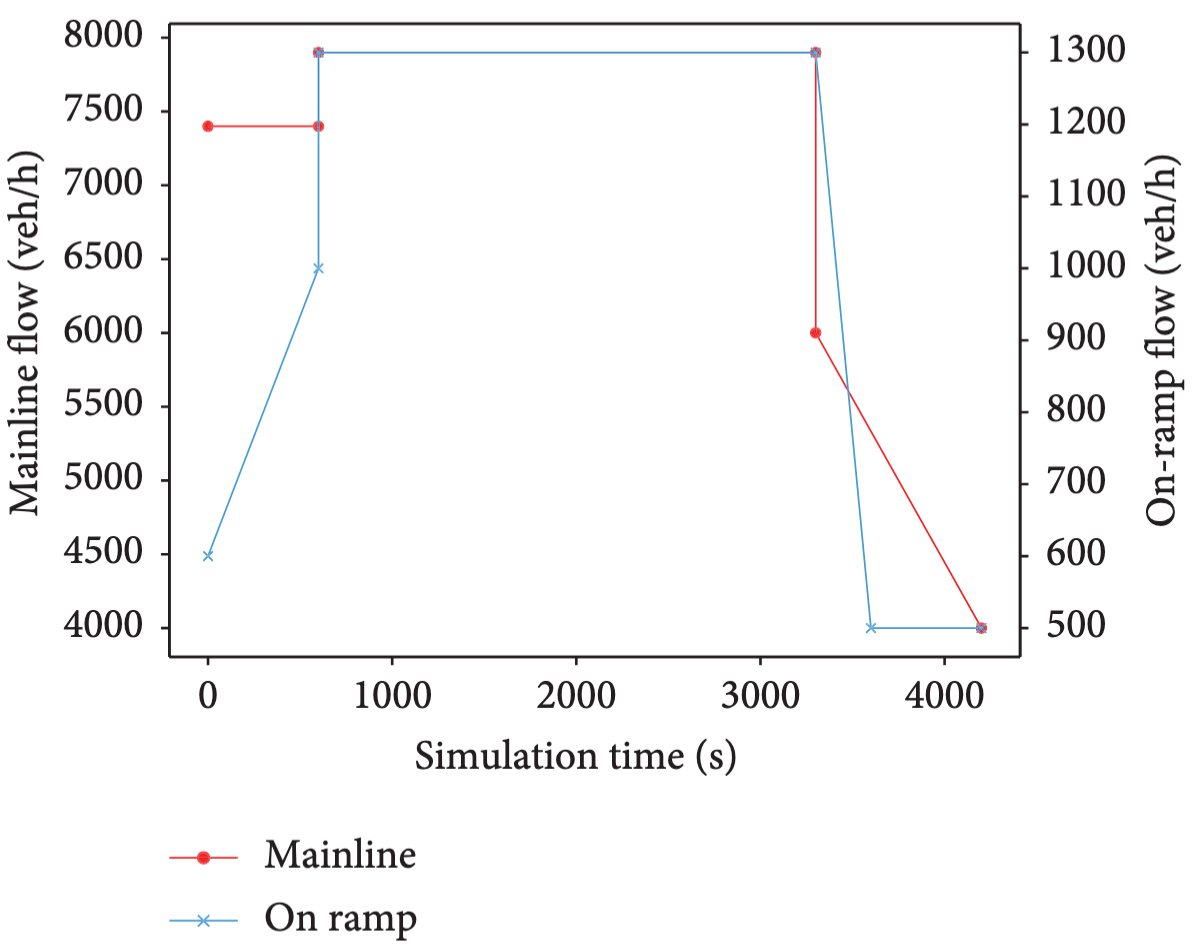
\includegraphics[width=0.6\linewidth]{figures/yang2025_fig5.png}
    \caption{Single-ramp input flow profile used in the replication. Original from~\cite{Yang2025Reinforcement}, Figure~5.}
    \label{fig:single_ramp_demand}
\end{figure}

The exact demand values extracted from the original figure were used without adjustment. Under this profile, the reconstructed simulation produced no ramp queue spillback and only mild congestion, with TTS values below those reported in the original study. All single-ramp results in this report use this paper-reported demand profile, referred to as Demand~A.


SUMO vehicle and driver parameters were adopted from Table~2 of the original paper and are listed in Appendix~\ref{sec:implementation_parameters}.

% Ramp 1: 32°02'11.8"N 118°52'40.0"E
% Last Ramp: 32°00'12.6"N 118°50'12.1"E
\paragraph{Multi-Ramp Scenario.}\label{sec:impl_multi_ramp} 
The multi-ramp scenario replicates a 7.64~km section of the Nanjing Ring Expressway (spanning from 32$^\circ$02'11.8''N, 118$^\circ$52'40.0''E at Ramp~1 to 32$^\circ$00'12.6''N, 118$^\circ$50'12.1''E at Ramp~4) containing four on-ramps: Maqun South Road (Ramp~1), Shuangqi Road (Ramp~2), Shiyang Road (Ramp~3), and Inner Ring South Line (Ramp~4), and their respective off-ramps. The network geometry was reconstructed from Figure~11 of the original paper. The mainline has four lanes with a capacity of 8{,}100~veh$\cdot$h. Per-ramp capacities and maximum queue lengths are listed in Table~\ref{tab:ramp_params}.

\begin{figure}[!h]
    \centering
    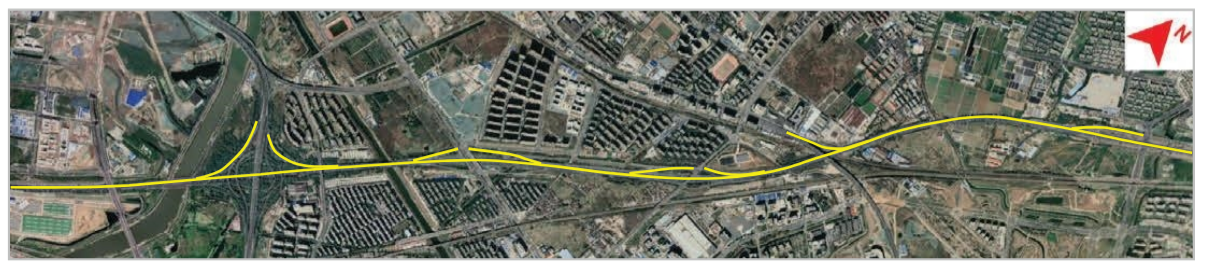
\includegraphics[width=0.9\linewidth]{figures/yang2025_fig11.png}\\[0.5em]
    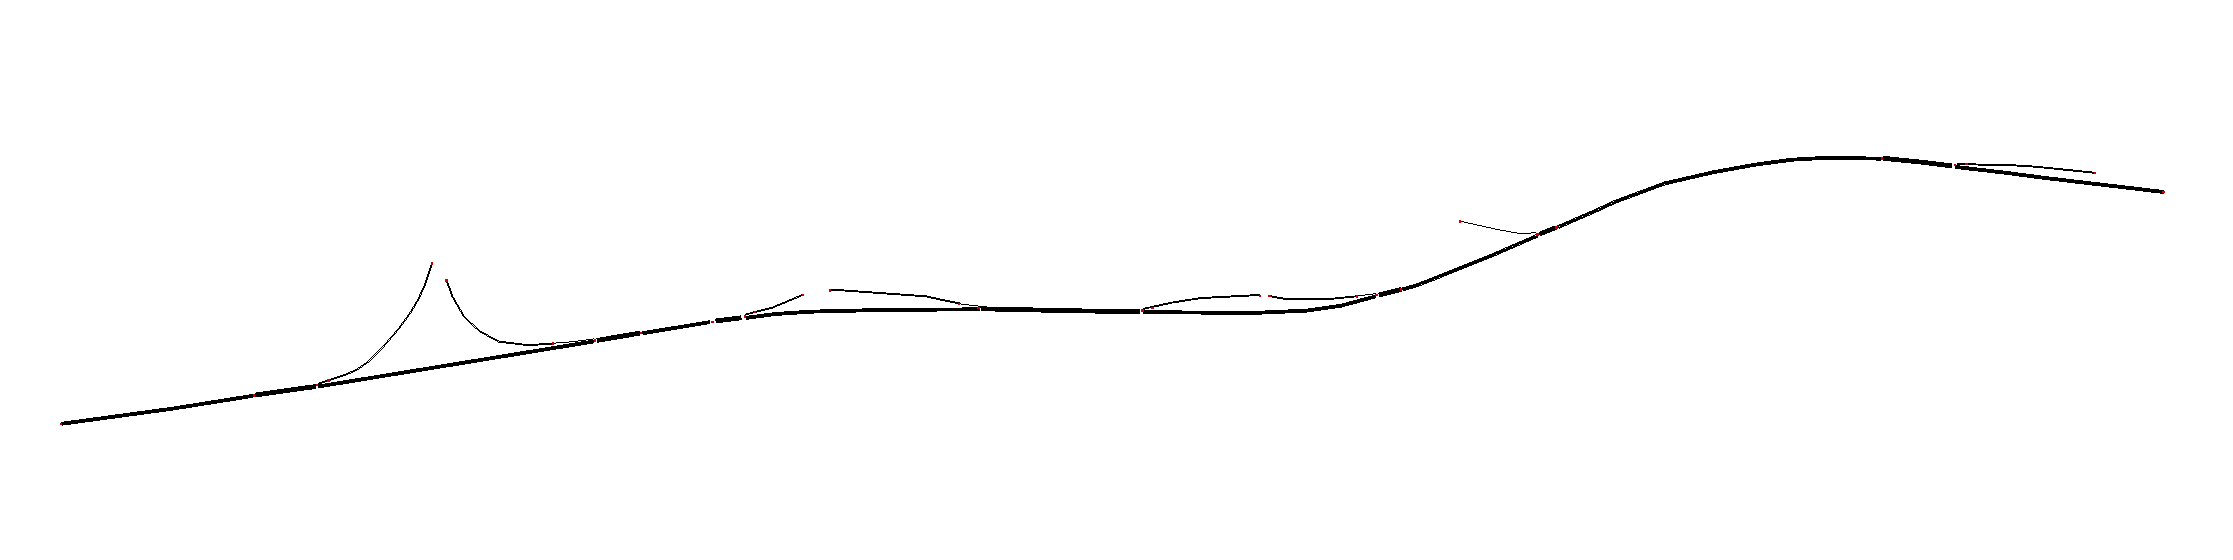
\includegraphics[width=0.9\linewidth]{figures/yang2025_fig11_rep.png}
    \caption{Satellite map of the multi-ramp test corridor on the Nanjing Ring Expressway. Top: original from~\cite{Yang2025Reinforcement}, Figure~11. Bottom: reconstructed test segment used in the replication.}
    \label{fig:multi_ramp_map}
\end{figure}

The original paper reports a distance of 397~m between the Shiyang Road on-ramp and its downstream off-ramp. Satellite measurements instead indicated 571~m. The reconstructed network uses 571~m because shortening this distance would alter the overall network geometry.

The lane configurations at the merge zones were also ambiguous. Two reconstructed topologies, Scenarios~3 and~4, were tested. Scenario~3 produced an immediate network breakdown under the baseline demand. Scenario~4 was therefore used for all experiments. More detail provided in Appendix \ref{sec:appendix_capacity}.

\paragraph{Maximum ramp queue.}
The original paper does not specify the maximum queue storage capacity $w_{\max}$ for any of the four ramps. These values were determined empirically: the ramp traffic signal was held permanently at red while ramp demand was applied, and the simulation was run until queue growth stopped. The number of vehicles accumulated on the ramp storage area at steady state was recorded as $w_{\max}$. The measured values of 84, 112, 58, and 164 vehicles for Ramps 1--4, respectively, are replication-specific assumptions.

\paragraph{Ramp capacity.}
The original paper reports per-ramp capacities of 2{,}540, 2{,}650, 1{,}930, and 2{,}300~veh$\cdot$h for ramps~1--4 respectively. To verify this, ramp demand was varied from 1{,}800 to 2{,}300~veh$\cdot$h in steps of 50~veh$\cdot$h, with mainline demand set to zero, as detailed in Appendix \ref{sec:appendix_capacity}. Ten simulations with different random seeds were run at each demand level. Persistent congestion was defined as a queue exceeding 50\% of $w_{\max}$ for 20 consecutive control steps. The resulting capacities---1{,}900, 1{,}850, 1{,}850, and 1{,}950~veh$\cdot$h---were substantially below the reported values. The reported values were nevertheless used as the nominal capacity $C$ in the action replacement formula.

\begin{table*}[!h]
    \centering
    \caption{Multi-ramp scenario: paper-reported and empirically measured per-ramp capacities, and maximum queue storage determined by red-light experiment. The paper does not report $w_{\max}$.}
    \label{tab:ramp_params}
    \begin{tabular}{llrrr}
    \toprule
    \textbf{Ramp} & \textbf{Name} & \thead{\textbf{Paper cap.}\\\textbf{(veh$\cdot$h)}} & \thead{\textbf{Measured cap.}\\\textbf{(veh$\cdot$h)}} & \thead{\textbf{$w_{\max}$}\\\textbf{(veh)}} \\
    \midrule
    Ramp~1 & Maqun South Road      & 2{,}540 & 1{,}900 & 84 \\
    Ramp~2 & Shuangqi Road         & 2{,}650 & 1{,}850 & 112 \\
    Ramp~3 & Shiyang Road          & 1{,}930 & 1{,}850 & 58 \\
    Ramp~4 & Inner Ring South Line & 2{,}300 & 1{,}950 & 164 \\
    \bottomrule
    \end{tabular}
\end{table*}

While the original study provides downstream traffic flow for each on-ramp (Figure~\ref{fig:multi_ramp_demand}), it does not provide the mainline and ramp demand series or account for flow leaving through the four off-ramps. Constant demands were therefore estimated as 8{,}000~veh$\cdot$h for the mainline and 1{,}400, 1{,}200, 900, and 1{,}600~veh$\cdot$h for ramps~1--4. The simulation step and control interval remained 1~s and 15~s, respectively. Multi-ramp episodes ran for 320 control steps (4{,}800~s).

\begin{figure}[!h]
    \centering
    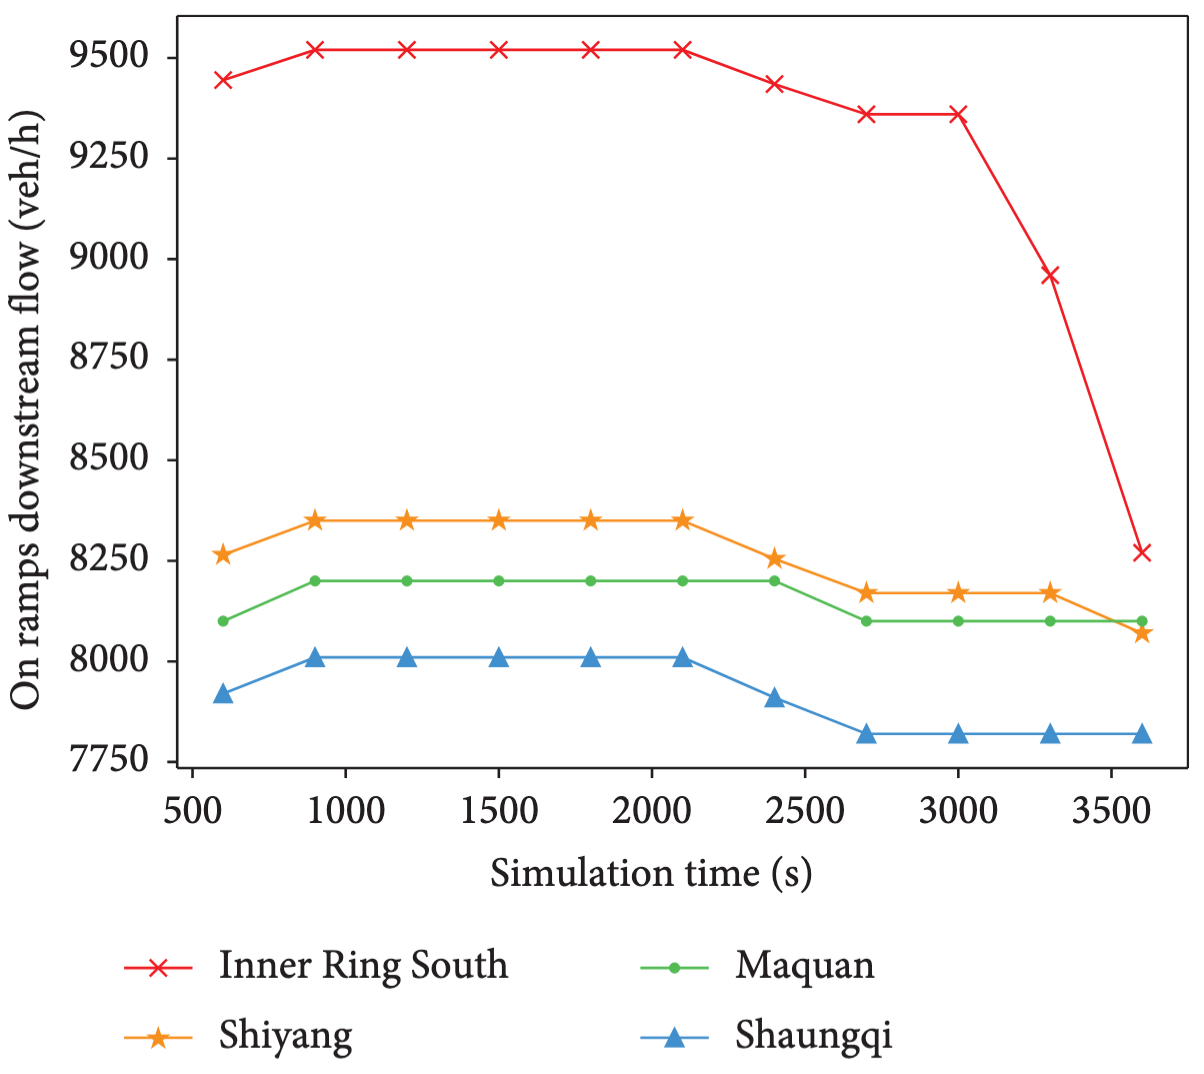
\includegraphics[width=0.6\linewidth]{figures/yang2025_fig12.png}
    \caption{Downstream traffic flow per on-ramp in the multi-ramp scenario. Original from~\cite{Yang2025Reinforcement}, Figure~12.}
    \label{fig:multi_ramp_demand}
\end{figure}

To ensure fidelity to the original simulation environment, these demand parameters were iteratively fine-tuned. Because exact numerical errors could not be calculated against the original data, calibration relied on visual comparison with the spatiotemporal speed diagrams published in the reference study (Figure~\ref{fig:demand_calibration_heatmap}). Specifically, the baseline demand was adjusted to align with the original study's observation that congestion under the no-control strategy ``starts to form downstream around 1500~s, and the congestion gradually spreads from the downstream of the Inner Ring South Line to the Maqun South Road from 2500~s, forming large-scale congestion in the weaving area between Shuangqi Road and Shiyang Road''~\cite{Yang2025Reinforcement}.

The reconstructed network was instrumented with induction-loop detectors at 50~m intervals. Mean speed across all lanes was aggregated every 15~s to form a space--time speed matrix. Demand values were tuned by comparing the approximate congestion onset time and upstream propagation direction with the no-control panel of Figure~15 in the original study.

\begin{figure*}[!h]
    \centering
    \begin{subfigure}[b]{0.47\textwidth}
        \centering
        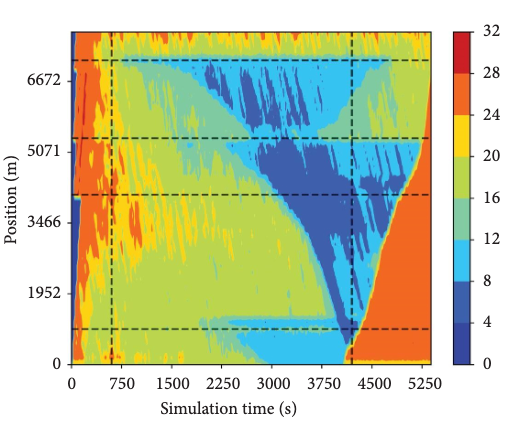
\includegraphics[width=\textwidth]{figures/yang2025_fig15a.png}
        \caption{Original study}
    \end{subfigure}
    \hfill
    \begin{subfigure}[b]{0.47\textwidth}
        \centering
        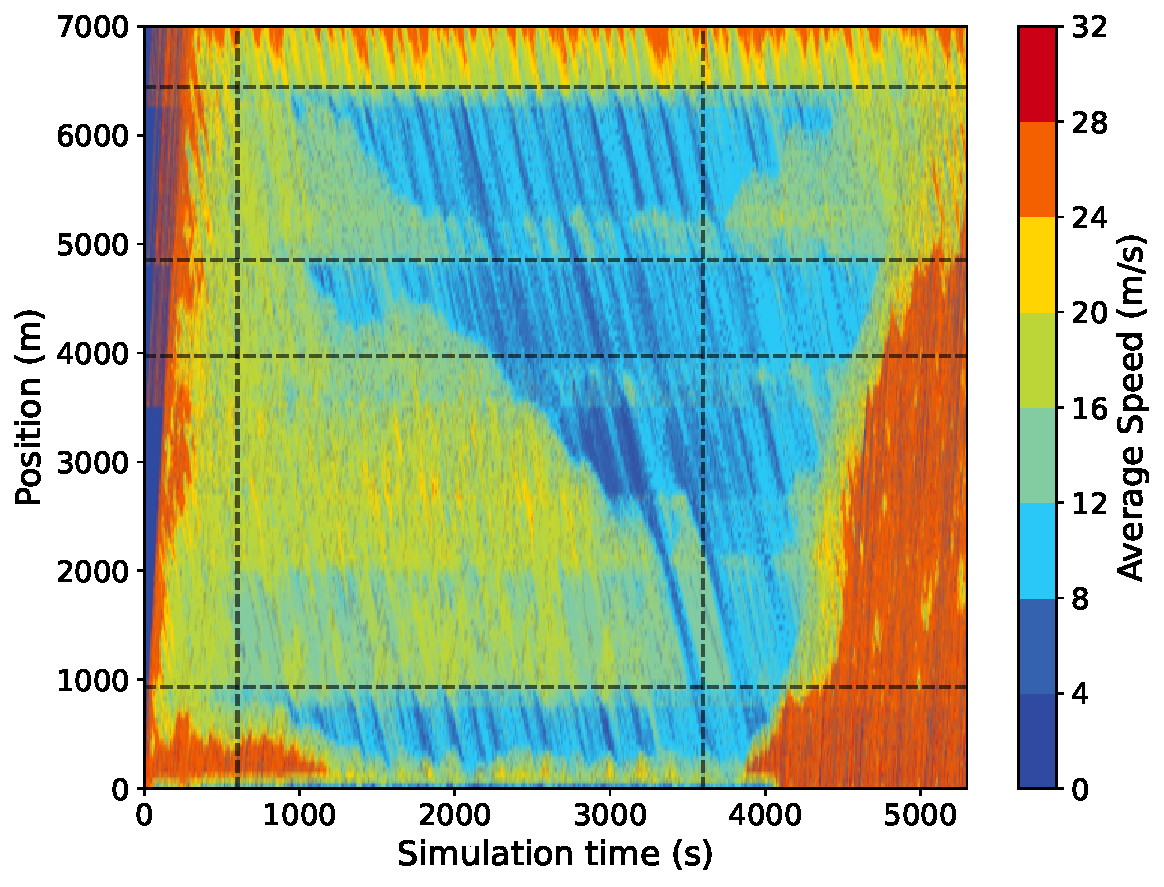
\includegraphics[width=\textwidth]{figures/fig_15a_rep.pdf}
        \caption{Replication}
    \end{subfigure}
    \caption{No-control space--time speed heatmaps used for multi-ramp demand calibration. The comparison was qualitative because the original numerical data were unavailable.}
    \label{fig:demand_calibration_heatmap}
\end{figure*}

The reconstructed network reproduced the approximate congestion onset and propagation direction, but not the spatial extent, intensity, or the reported propagation from Ramp~4 to Ramp~3. The calibration is therefore qualitative rather than an exact reconstruction.


\subsection{Benchmark Controllers}

The proposed RL agent was compared to different baseline controllers in both scenarios.

\subsubsection{No-Control Baseline}

In the no-control (NC) scenario all ramp traffic signals remain green throughout the simulation (metering ratio fixed at 1.0 for every ramp and every control step). The NC scenario was executed prior to training to measure the step-wise TTS distribution, which provides the calibration constants for the reward function (Section~\ref{sec:reward}).

\subsubsection{PI-ALINEA}

PI-ALINEA is a proportional-integral extension of the ALINEA ramp-metering law~\cite{Papageorgiou1991ALINEA} that regulates on-ramp inflow via downstream occupancy feedback. Following Eq.~(16) of~\cite{Yang2025Reinforcement}, the control law is
\[
r(k) = r(k-1) + \frac{k_r}{C}\bigl(\hat{o} - o(k)\bigr) - \frac{k_p}{C}\bigl(o(k) - o(k-1)\bigr),
\]
where $r(k)$ is the metering ratio at control step $k$, $C$ is the ramp capacity (veh$\cdot$h), $\hat{o}$ is the target downstream occupancy (\%), $o(k)$ is the measured downstream occupancy, and $k_r$, $k_p$ are the proportional and integral gains. The output is clipped to $[0.1,\, 1.0]$.

The critical occupancy for the single-ramp scenario was set to $\hat{o}=14\%$, consistent with Figure~7 of the original paper. All gain values were adopted directly from the original paper and are listed in Appendix~\ref{sec:implementation_parameters}.

\begin{figure}[!h]
    \centering
    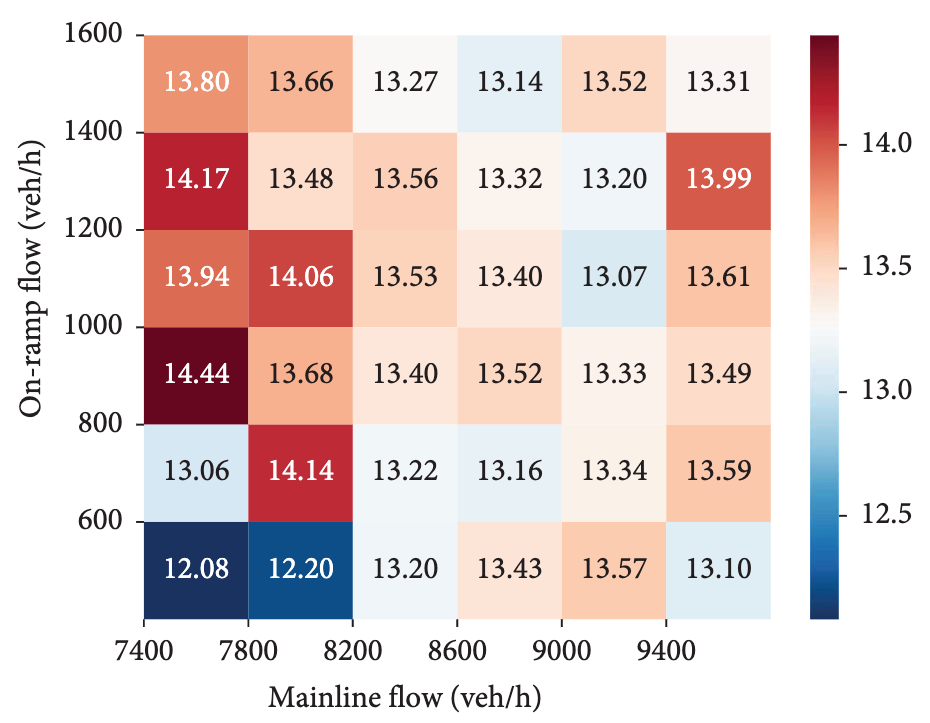
\includegraphics[width=0.7\linewidth]{figures/yang2025_fig7.png}
    \caption{Downstream occupancy variation used to determine the critical occupancy threshold ($\hat{o} = 14\%$) for the single-ramp PI-ALINEA controller. Reproduced from~\cite{Yang2025Reinforcement}, Figure~7.}
    \label{fig:occ_analysis}
\end{figure}

\subsubsection{HERO}

HERO~\cite{Papamichail2010HERO} coordinates PI-ALINEA controllers across the four-ramp network by recruiting upstream ramps when a downstream queue becomes critical. Each ramp normally operates its own local PI-ALINEA regulator. When a ramp's queue occupancy exceeds the activation threshold $q_\mathrm{on}$, the controller enters an emergency state: the immediately upstream ramp is recruited as a ``slave'' and its metering rate is reduced to divert demand away from the critical ramp. This coordination cascades upstream if the queue continues to grow, and is released once the queue occupancy falls below the deactivation threshold $q_\mathrm{off}$, restoring independent local control.

The original study does not report its queue thresholds or the precise recruitment logic used for the four-ramp network. Following general rule-based coordination principles, we adopted an activation threshold of $q_{\mathrm{on}}=0.5$, a deactivation threshold of $q_{\mathrm{off}}=0.3$, and a minimum slave metering rate of $q_{\mathrm{slave}}=0.2$ as heuristic defaults for this replication. Using distinct thresholds for activation and deactivation prevents rapid switching between local and coordinated control at the threshold boundary.


\subsection{RL Agent Design}

\subsubsection{Network Architecture}

The PPO actor and critic use a shared feature extractor followed by separate heads, following the structure reported by Yang et al~\cite{Yang2025Reinforcement}. The original study does not report the layer widths, actor output activation, or policy variance initialisation. We used 256-unit hidden layers and a Sigmoid actor output. The remaining architecture choices are listed in Appendix~\ref{sec:assumptions}.

\subsubsection{State Representation}

    The state vector is assembled from induction-loop measurements collected over each 15~s control interval.

    In the \textbf{single-ramp} scenario, the state is a 10-dimensional vector: three mainline upstream features (occupancy, mean speed, vehicle count), three mainline downstream features (occupancy, mean speed, vehicle count), and four ramp features (queue length, vehicle arrivals, vehicle departures, green duration in the previous control step).

    The paper does not specify the state dimensionality for the \textbf{multi-ramp} scenario. We used a 28-dimensional vector instead. For each of the four ramps, seven features are concatenated: downstream occupancy, downstream speed, downstream vehicle count, ramp queue length, ramp arrivals, ramp departures, and the previous metering ratio. Upstream mainline features are not included.

    Each feature is standardised before being fed to the network:
    \[
    \tilde{s} = \frac{s - \bar{s}}{\sigma_s},
    \]
    where $\bar s$ and $\sigma_s$ denote the mean and standard deviation of the feature $s$, respectively. The original study does not state whether these statistics are updated during training or computed from a fixed baseline. We tested both approaches and found no meaningful difference across multiple seeds. Fixed statistics computed from the no-control baseline were used in the final implementation; the comparison is shown in Appendix~\ref{sec:normalisation}.

\subsubsection{Action Space}

    The action is a continuous metering ratio $a \in [0,1]$, representing the fraction of the 15~s control step during which the ramp signal is green. This is equivalent to expressing the metering rate as a fraction of ramp capacity, consistent with the original paper.

    In the single-ramp scenario the action is a scalar. In the multi-ramp scenario the agent outputs a 4-dimensional vector (one ratio per ramp) sampled from a joint Normal distribution with diagonal covariance. A single centralised agent controls all four ramps simultaneously, as described in the original paper.

\subsubsection{Reward Function}
    \label{sec:reward}

    The step reward is a normalised measure of network efficiency based on the total time spent (TTS), following Eq.~(11) of~\cite{Yang2025Reinforcement}:
    \[
    \text{reward}(k) = \frac{A_{\mathrm{TTS}} - \mathrm{TTS}(k)}{B_{\mathrm{TTS}}},
    \]
    where $\mathrm{TTS}(k)$ is calculated by adding up the number of active vehicles at each second of control step $k$, $A_{\mathrm{TTS}}$ is the maximum step TTS observed under the no-control baseline, and $B_{\mathrm{TTS}}$ is the mean step TTS under the same baseline. The TTS computation includes vehicles waiting to enter the network at the end of each control step (pending vehicles). The calibrated constants are:

    % ASSUMPTION

    \begin{itemize}
        \item Single-ramp: $A_{\mathrm{TTS}} = 11{,}135.0$, $B_{\mathrm{TTS}} = 6{,}774.73$.
        \item Multi-ramp: $A_{\mathrm{TTS}} = 24{,}372.40$, $B_{\mathrm{TTS}} = 18{,}296.09$.
    \end{itemize}

    When the action replacement module is active and the agent's action is overridden, the reward is further modified as described in Section~\ref{sec:penalty}.


\subsection{Action Replacement Module}

The action replacement module enforces the queue-spillback constraint during training by overriding actions below the computed safe lower bound, as summarised in Figure~\ref{fig:method_summary}.

\subsubsection{Lower Bound Computation}

At each control step $k$, a metering-rate lower bound is derived from the store-and-forward model to prevent queue overflow. Following Eqs.~(12)--(13) of~\cite{Yang2025Reinforcement}:
\[
a_{\mathrm{lb}}(k) = \max\!\left\{ a_{\min},\; \frac{d(k-1) - \dfrac{\alpha \cdot w_{\max} - w(k)}{T}}{C} \right\},
\]
where $d(k-1)$ is the previous-step ramp demand (veh$\cdot$s), $w(k)$ is the current queue length (veh), $w_{\max}$ is the maximum ramp storage (veh), $C$ is the ramp capacity (veh$\cdot$s), $T = 15$~s is the control step length, and $a_{\min} = 0.1$ is the minimum allowable metering ratio. The coefficient $\alpha$ limits the queue target to $\alpha \cdot w_{\max}$, providing a safety margin. The original paper states $\alpha < 1$ without giving a numerical value; $\alpha = 0.9$ was used in the replication. The bound is clamped to $[a_{\min},\, 1]$.

If the agent's action $a(k) < a_{\mathrm{lb}}(k)$ and the replacement mechanism is enabled, the executed action is set to $a_{\mathrm{lb}}(k)$.

\subsubsection{Penalty Calculation and Reward Modification}
\label{sec:penalty}

When an action is replaced at step $k$, the reward is penalised following Eqs.~(14)--(15) of~\cite{Yang2025Reinforcement}:
\[
R(k) = \text{reward}(k) - c \cdot \mathrm{penalty}(k),
\]
where $\text{reward}(k)$ is the base step reward (Section~\ref{sec:reward}) and the penalty is
\[
\mathrm{penalty}(k) = \frac{w(k)}{k_{\mathrm{sp}} + 1},
\]
with $k_{\mathrm{sp}}$ the predicted number of control steps remaining until spillback:
\[
k_{\mathrm{sp}} = \max\!\left\{1,\; \frac{\alpha \cdot w_{\max} - w(k)}{\bigl(d(k) - a(k) \cdot C\bigr) \cdot T}\right\}.
\]
If the net accumulation rate is non-positive ($d(k) \le a(k) \cdot C$), the penalty is zero. The scaling factor $c$ is not reported in the original paper; $c = 0.1$ was used in the replication.


\subsection{Training Pipeline}

\subsubsection{PPO Algorithm and Hyperparameters}
\label{sec:ppo}

The PPO agent was implemented from scratch in PyTorch using the clipped PPO objective, generalised advantage estimation, a value loss, and entropy regularisation~\cite{Schulman2015GAE}. The original paper does not report its training hyperparameters. The adopted values are listed in Appendix~\ref{sec:implementation_parameters}.

The original paper employs a vectorised environment architecture consisting of $N$ parallel SUMO instances to accelerate trajectory data collection, as depicted in Figure~3 of~\cite{Yang2025Reinforcement}. In a standard vectorised setup, a single central agent processes batched states from multiple independent simulations simultaneously. However, the original study does not specify the exact number of parallel instances ($N$) utilised, nor does it detail how these parallel trajectories are aggregated into the rollout buffer for policy updates.

To avoid introducing unverified architectural complexity, this replication uses one sequential environment ($N=1$). Policy updates use one complete episode without mini-batch shuffling.

\subsection{Experimental Protocol}

Single-ramp training and evaluation used only the demand profile reported in the original paper (Demand~A). Controller performance was evaluated across ten independent random seeds (0--9), and results are reported as means with standard deviations. The multi-ramp capacity tests likewise used ten seeds for each demand level. During evaluation, the learned policy mean was used instead of sampling from the training distribution.


\subsection{Assumptions}

A full list of all assumptions made during this replication can be found in Appendix \ref{sec:assumptions}.

\section{Results \& Discussion}
\label{sec:results}

Replicated results are compared directly with the figures and metrics reported by Yang et al~\cite{Yang2025Reinforcement}. Unless stated otherwise, discrepancies are attributed to the network geometry, demand profiles, and capacity parameters that were unavailable and therefore reconstructed or estimated, as described in Section~\ref{sec:implementation_details} and Appendix~\ref{sec:assumptions}.

\subsection{Single-Ramp Scenario}

\subsubsection{Network and Environment Properties}

\paragraph{Replication of Figure 6.} Figure~\ref{fig:single_ramp_fig6_rep} compares the modified cumulative arrival curves $N'(x,t)=N(x,t)-q_0t$ at three detector locations. The original study uses a background flow of $q_0=8{,}160$~veh$\cdot$h and reports capacity drops at approximately 600~s and 950~s. In the replication, the curves diverge gradually after the demand step at 600~s, but the sharp second drop is not reproduced. The vertical range also differs substantially. Because the background flow was calibrated for the original SUMO network, small differences in network geometry and capacity have a cumulative effect on these curves.

\begin{figure}[!h]
    \centering
    \begin{subfigure}[b]{0.48\linewidth}
        \centering
        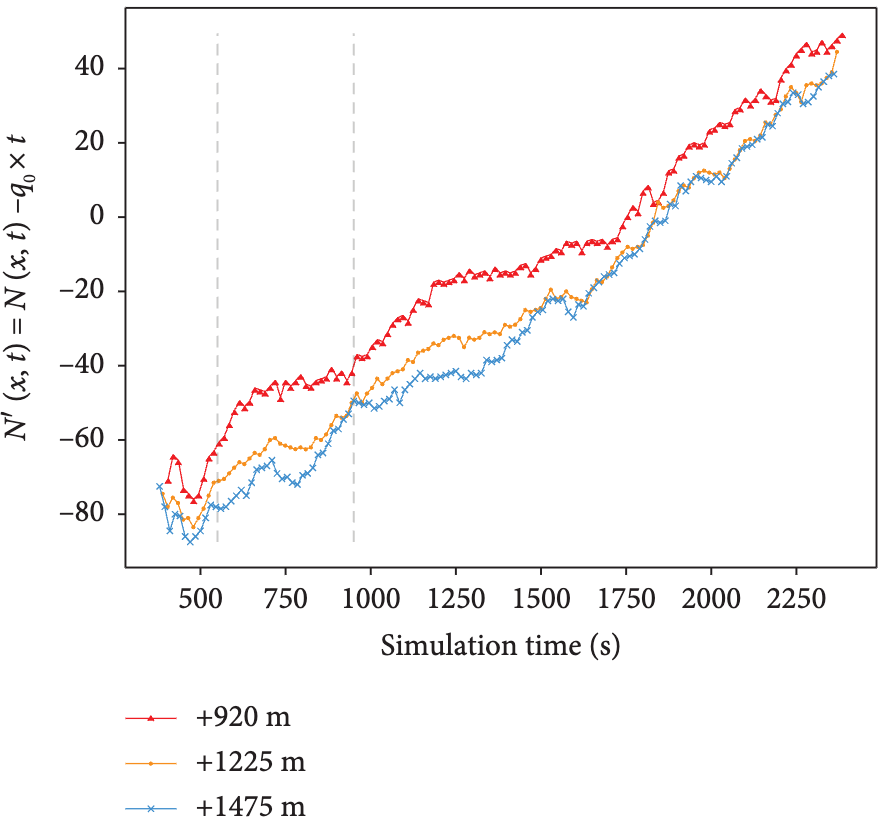
\includegraphics[width=\linewidth]{figures/yang2025_fig6.png}
        \caption{Original study}
        \label{fig:fig6_orig}
    \end{subfigure}
    \hfill
    \begin{subfigure}[b]{0.48\linewidth}
        \centering
        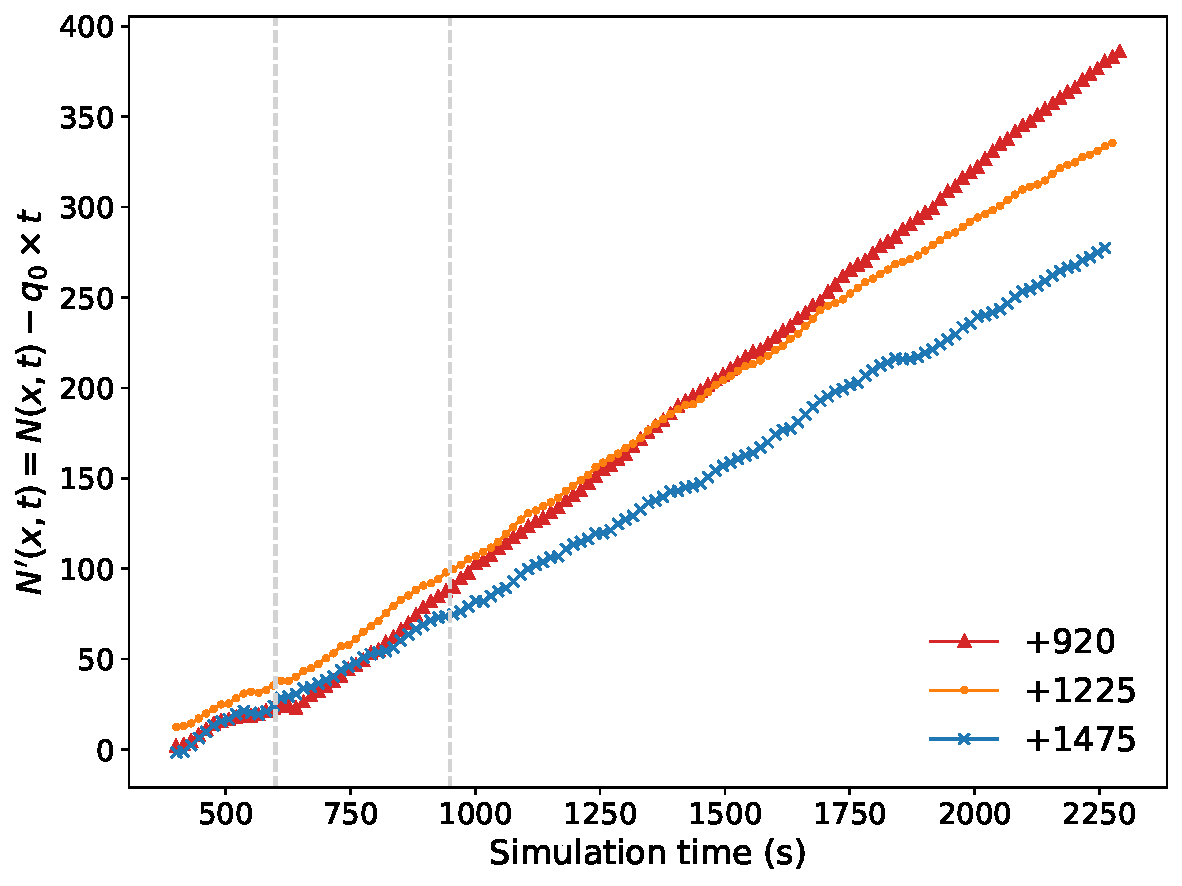
\includegraphics[width=\linewidth]{figures/fig_6_rep.pdf}
        \caption{Replicated study}
        \label{fig:fig6_rep}
    \end{subfigure}
    \caption{Modified cumulative arrival curves $N'(x,t)$ at three detector locations (upstream at $+920$~m, downstream at $+1225$~m and $+1475$~m) in the single-ramp corridor, corresponding to Figure~6 of~\cite{Yang2025Reinforcement}. The original paper (a) shows two distinct capacity-drop events at $\approx600$~s and $\approx950$~s; the replication (b) shows only a gradual, steady divergence after 600~s with no sharp secondary drop.}
    \label{fig:single_ramp_fig6_rep}
\end{figure}

\paragraph{Replication of Figure 7.} A comparison between the replicated downstream occupancy matrix and the original study's results highlights significant discrepancies in network behaviour under identical nominal demands (see Figure~\ref{fig:single_ramp_fig7_rep}). In the original study (Figure~\ref{fig:single_ramp_fig7_rep}, left), the occupancy matrix lacks a monotonic gradient; counter-intuitively, the highest combined demands (e.g., 9400\,veh$\cdot$h mainline and 1600\,veh$\cdot$h ramp) yield lower downstream occupancies than significantly lower demand configurations.

This pattern indicates an unmanaged upstream bottleneck or boundary gating effect in the original simulation setup. When input demand exceeds the network's physical capacity, vehicles queue at the insertion points outside the detector zone, causing downstream vehicle starvation and artificially lowering occupancy readings. Furthermore, the localised peak of 14.44\% at low-demand inputs suggests that the original results may suffer from stochastic noise, potentially due to evaluating an insufficient number of random seeds.

In contrast, the replicated network (Figure \ref{fig:single_ramp_fig7_rep}, right) exhibits consistently higher occupancy values across the entire matrix, varying narrowly between 14.60\% and 16.78\%. This uniformity indicates that the reconstructed network operates at or near capacity across the entire tested flow range. The absence of a low-occupancy blue zone in the bottom-left quadrant confirms that even the baseline demands are sufficient to saturate the merge area under the reconstructed geometry and default SUMO lane-changing dynamics. This critical difference underscores the challenge of achieving exact macroscopic replication using only reported demand figures, as micro-simulation capacity is highly sensitive to undocumented network topology and connection constraints.

\begin{figure}[!h]
    \centering
    \begin{subfigure}[b]{0.48\linewidth}
        \centering
        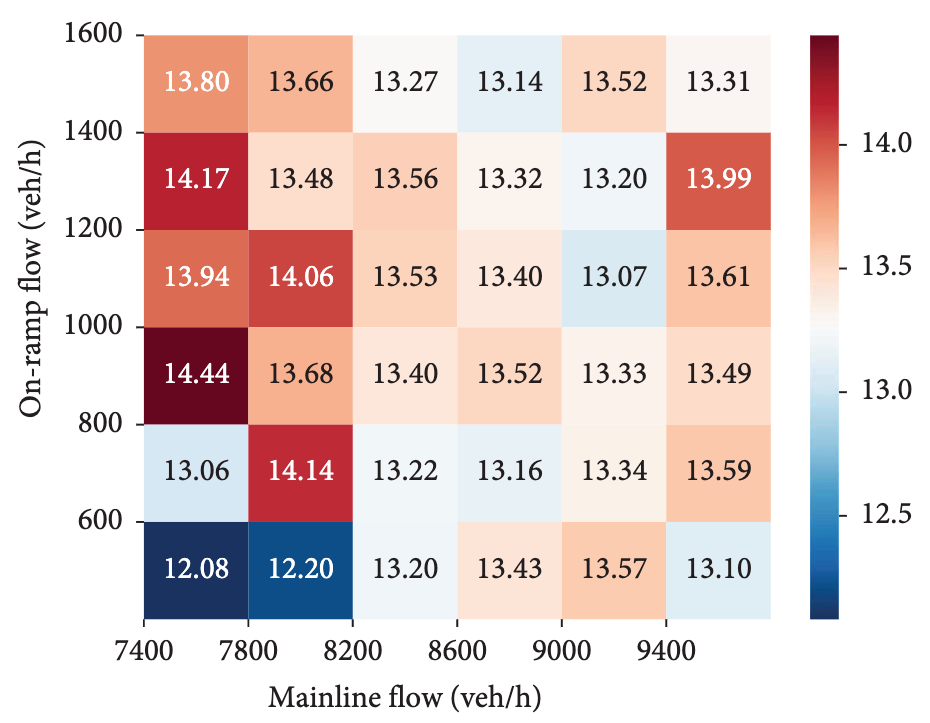
\includegraphics[width=\linewidth]{figures/yang2025_fig7.png}
        \caption{Original study}
        \label{fig:fig6_orig}
    \end{subfigure}
    \hfill
    \begin{subfigure}[b]{0.48\linewidth}
        \centering
        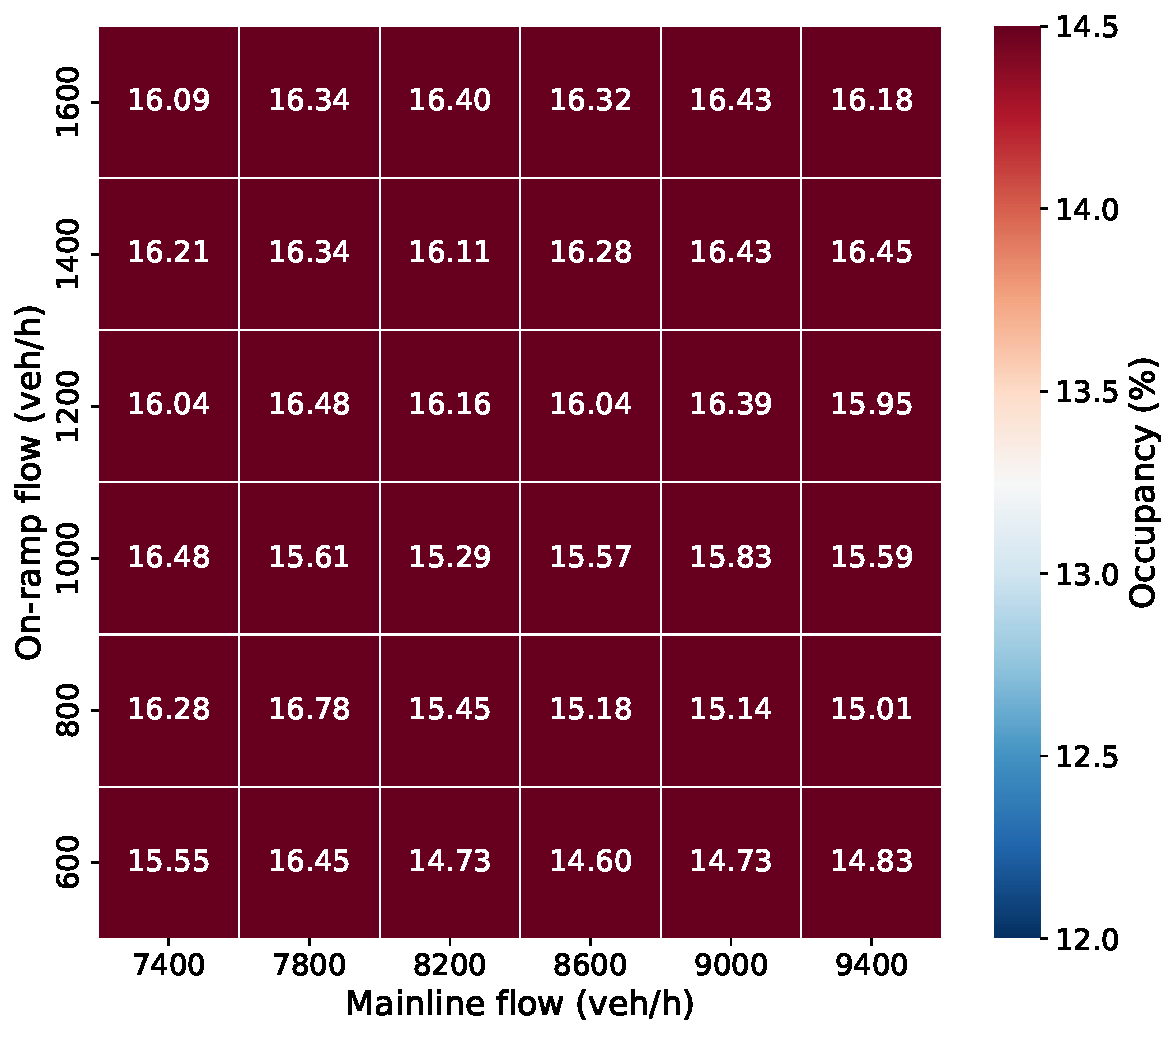
\includegraphics[width=\linewidth]{figures/fig_7_rep.pdf}
        \caption{Replicated study}
        \label{fig:fig6_rep}
    \end{subfigure}
    \caption{Downstream occupancy (\%) as a function of mainline and ramp inflow, corresponding to Figure~7 of~\cite{Yang2025Reinforcement}. The original paper shows a 12--13\% free-flow regime transitioning to $\approx14\%$ and capacity breakdown; the replication shows a uniformly $\approx14\%$ response across all flow combinations with no observable gradient.}
    \label{fig:single_ramp_fig7_rep}
\end{figure}

\subsubsection{Controller Performance}

A significant methodological limitation of the original study is that it does not report tabular TTS results for the safe RL controller. Regardless, we evaluated both the unconstrained agent and the agent with action replacement under the paper-reported single-ramp demand.

Table~\ref{tab:single_ramp_tts} compares the paper-reported TTS values against the mean and standard deviation obtained across ten independent simulation seeds (seeds 0--9) in this replication.

\begin{table*}[!h]
\centering
\caption{Single-ramp cumulative TTS in vehicle-hours (veh$\cdot$h) and percentage reduction relative to NC. Paper values are from Table~1 of~\cite{Yang2025Reinforcement}. Replication values use the paper-reported demand and are mean $\pm$ standard deviation over ten seeds.}
\label{tab:single_ramp_tts}
\begin{tabular}{lrrrr}
\toprule
& \multicolumn{2}{c}{\textbf{Original paper}} & \multicolumn{2}{c}{\textbf{Replication}} \\
\cmidrule(lr){2-3} \cmidrule(lr){4-5}
\textbf{Strategy} & \textbf{TTS (veh$\cdot$h)} & \textbf{Red.~(\%)} & \textbf{TTS (veh$\cdot$h)} & \textbf{Red.~(\%)} \\
\midrule
No Control (NC)                & 595.77 & --   & 446.94 $\pm$ 43.40 & -- \\
PI-ALINEA         & 578.27 & 2.94 & 443.27 $\pm$ 39.26 & 0.78 \\
RL                & 564.98 & 5.17 & 437.49 $\pm$ 41.02 & 2.11 \\
RL + Replacement  & N/A    & N/A  & 435.30 $\pm$ 40.25 & 2.56 \\
\bottomrule
\end{tabular}
\end{table*}

The qualitative ranking NC $>$ PI-ALINEA $>$ RL is preserved, but the replicated reductions are smaller. The seed-to-seed standard deviations of approximately 39--43~veh$\cdot$h are much larger than the mean differences between controllers. The mean difference between NC and PI-ALINEA is only 3.67~veh$\cdot$h, and some seeds show no improvement over NC. The original study reports neither a seed count nor uncertainty estimates, and its training figures show only single trajectories. The action replacement agent obtains a mean TTS of 435.30~veh$\cdot$h, compared with 437.49~veh$\cdot$h for the unconstrained agent. The original study does not report a corresponding TTS value for its safe controller.

The raw actions for seed~0 are shown in Figure~\ref{fig:agent_actions_demandA}. The policies behave similarly during the peak period but diverge near the end of the episode, when the action replacement agent meters the ramp more strongly.

\begin{figure}[!h]
\centering
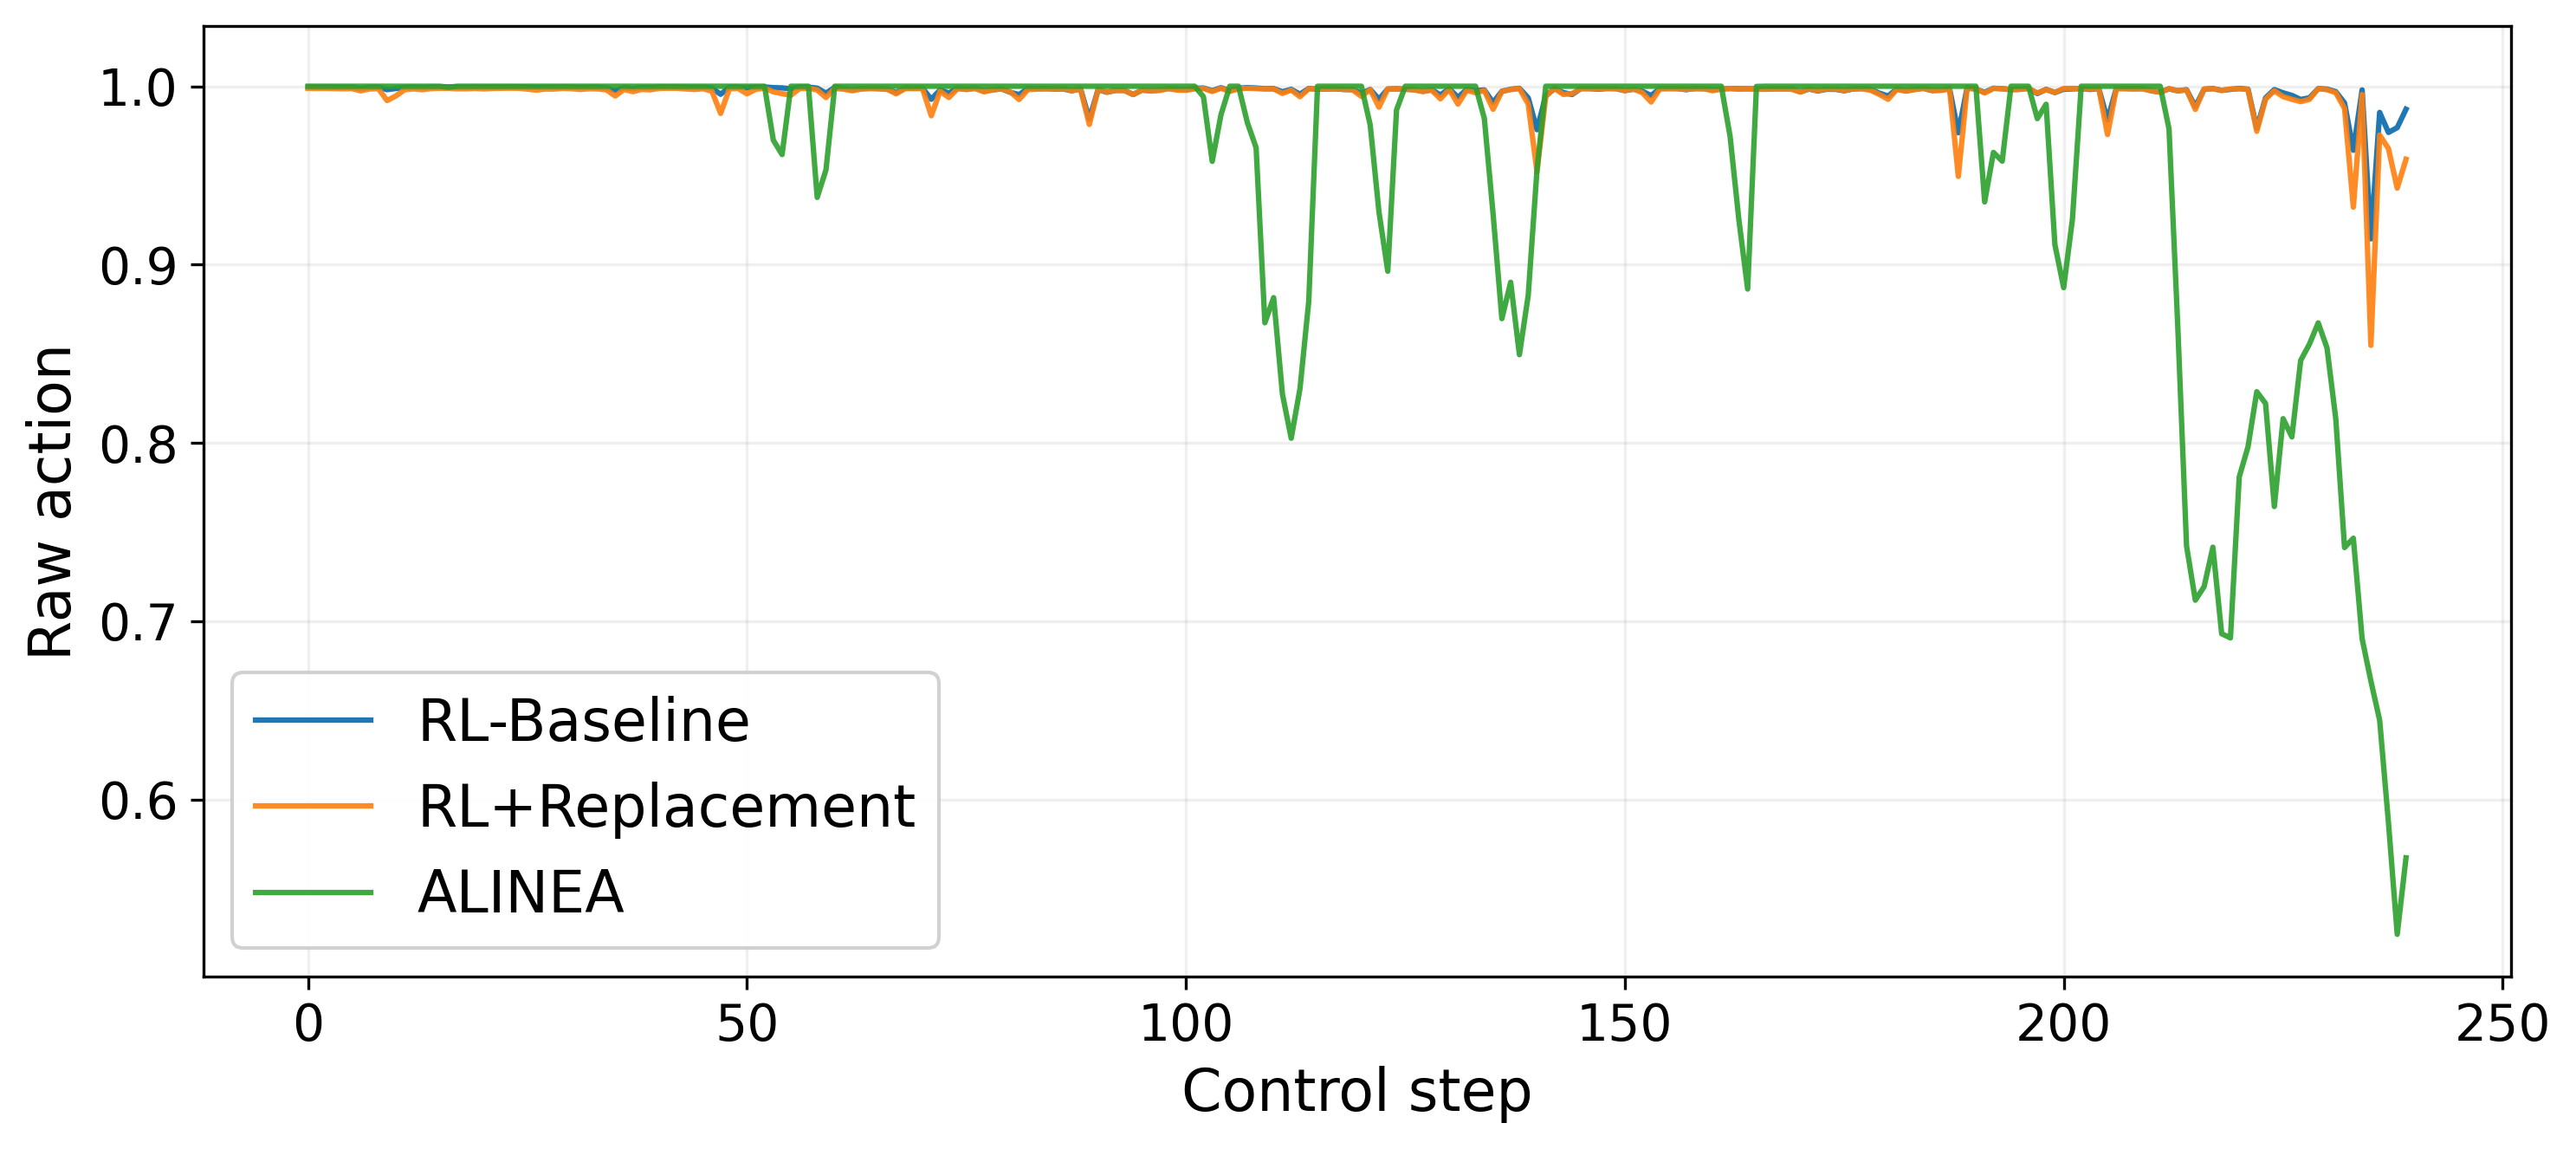
\includegraphics[width=1\linewidth]{figures/agent_actions_demandA.png}
\caption{Raw controller actions over time for Demand A (seed 0), comparing the baseline RL agent, the safe RL agent with action replacement, and PI-ALINEA. The safe policy demonstrates more aggressive metering restrictions during the low-demand recovery phase.}
\label{fig:agent_actions_demandA}
\end{figure}



\subsubsection{Training Dynamics and Action Replacement}
\label{sec:single_ramp_training}

\paragraph{Figures 8 and 9 Replication.} Figures \ref{fig:single_ramp_fig8_rep} and \ref{fig:single_ramp_fig9_rep} show the episode length and cumulative TTS per episode over the course of training, for the baseline agent (no lower bound constraint, orange) and the agent with the action replacement module (blue).

\begin{figure*}[h!]
    \centering
    \begin{subfigure}[t]{0.49\linewidth}
        \centering
        \subcaption*{Original}
        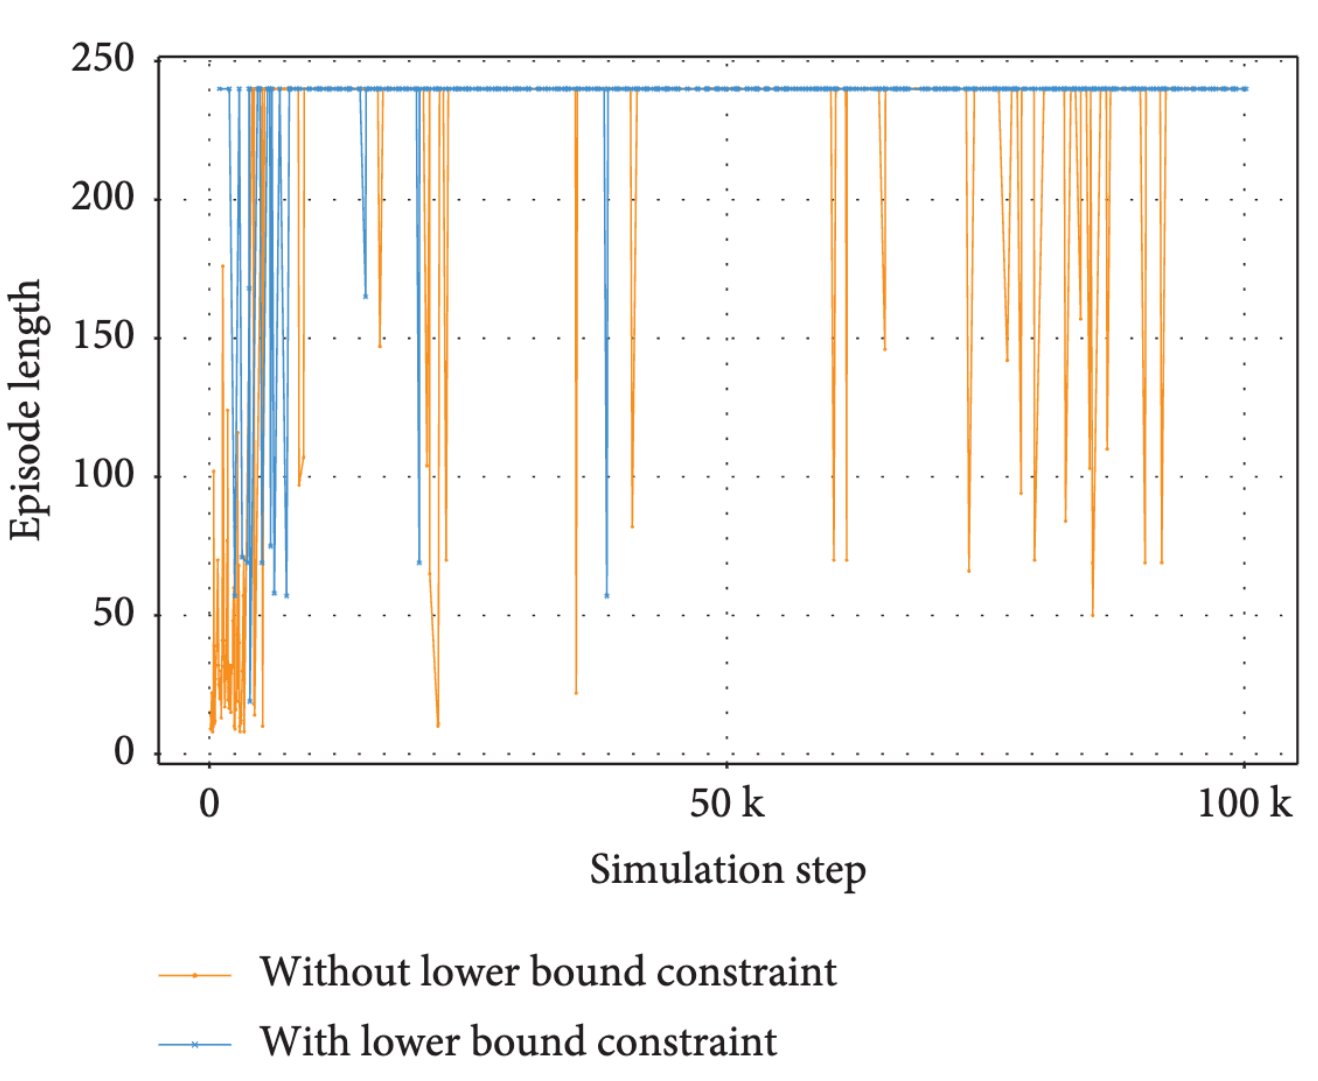
\includegraphics[width=0.95\linewidth]{figures/yang2025_fig8.png}
        \subcaption*{Replication}
        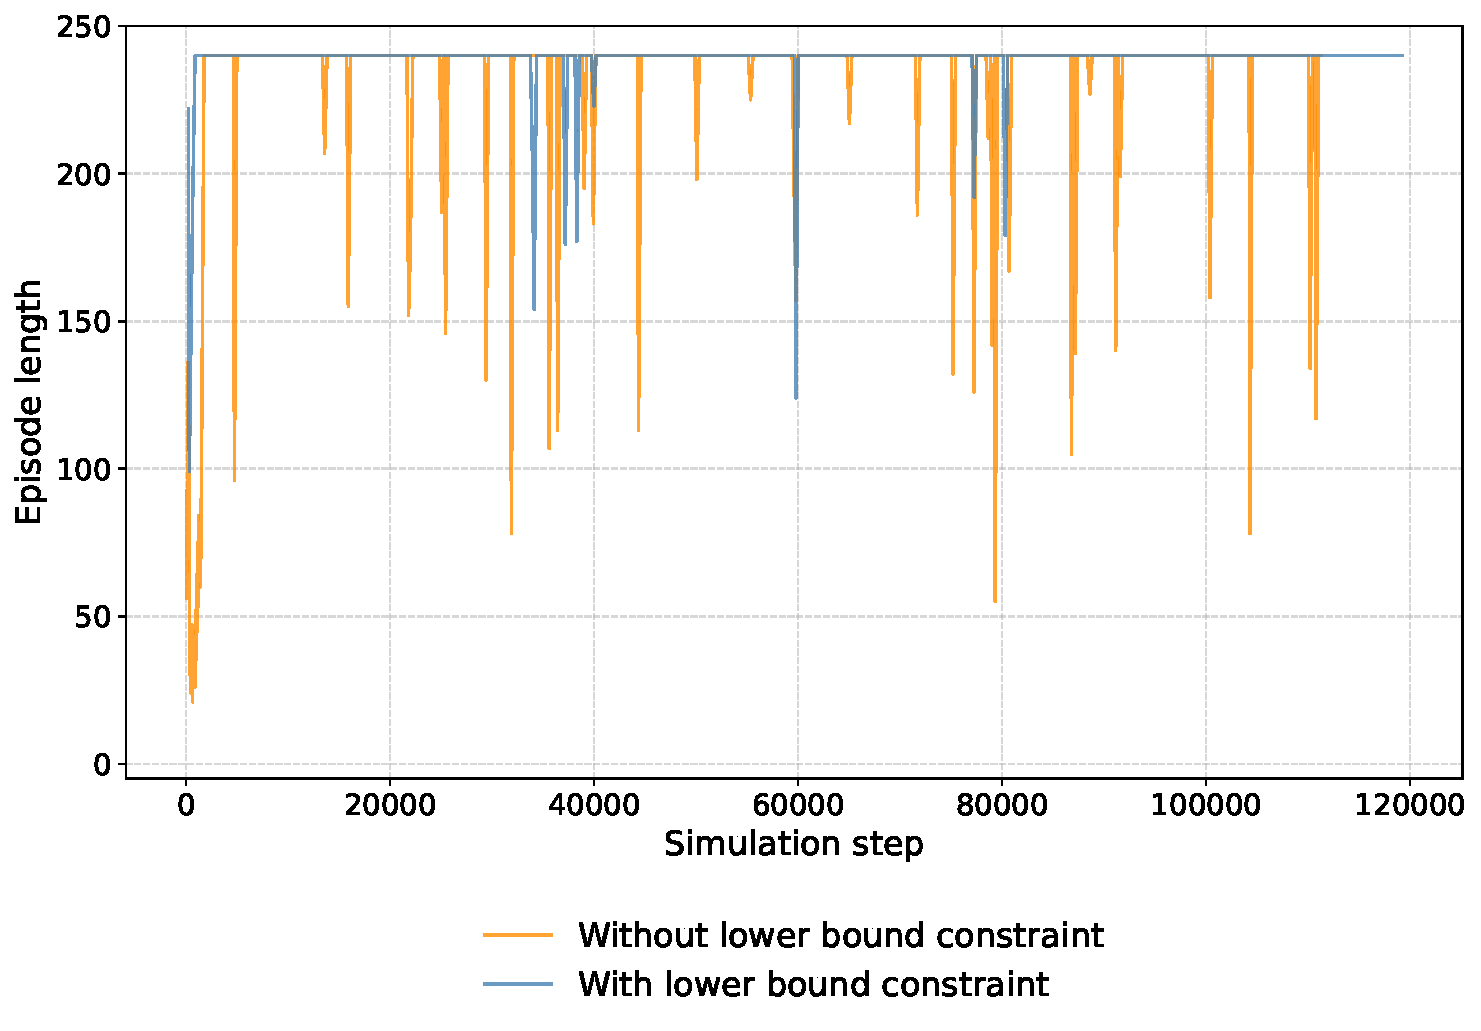
\includegraphics[width=0.95\linewidth]{figures/fig_8_rep.pdf}
        \caption{Episode length during training. Drops indicate early termination when $w>0.9 \cdot w_{\max}$.}
        \label{fig:single_ramp_fig8_rep}
    \end{subfigure}
    \hfill
    \begin{subfigure}[t]{0.49\linewidth}
        \centering
        \subcaption*{Original}
        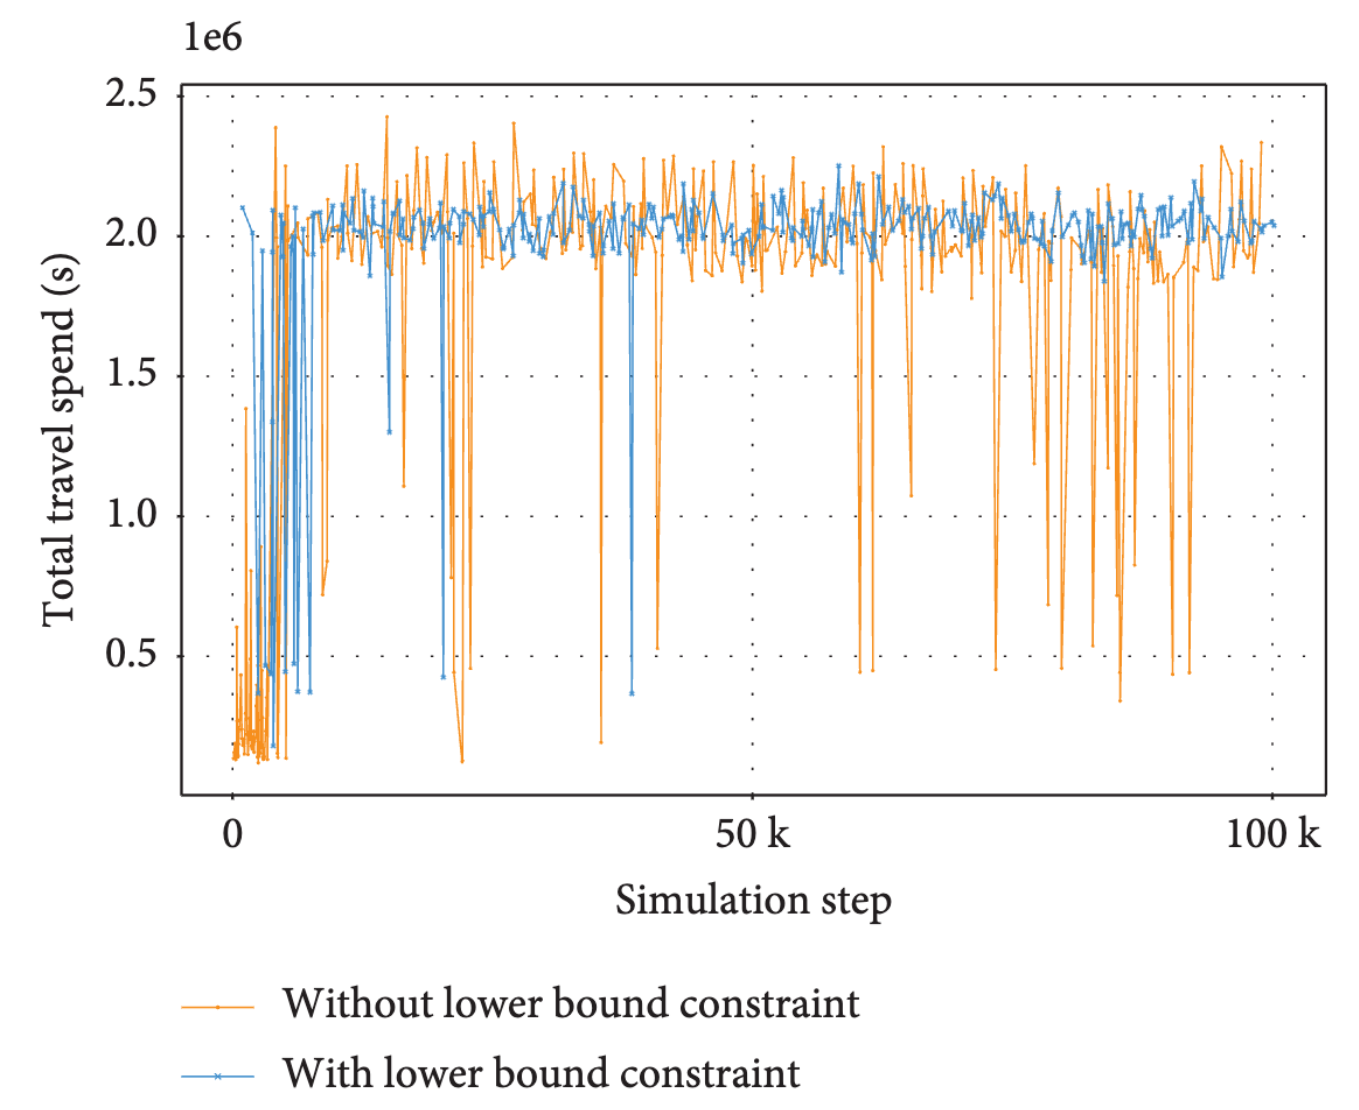
\includegraphics[width=0.95\linewidth]{figures/yang2025_fig9.png}
        \subcaption*{Replication}
        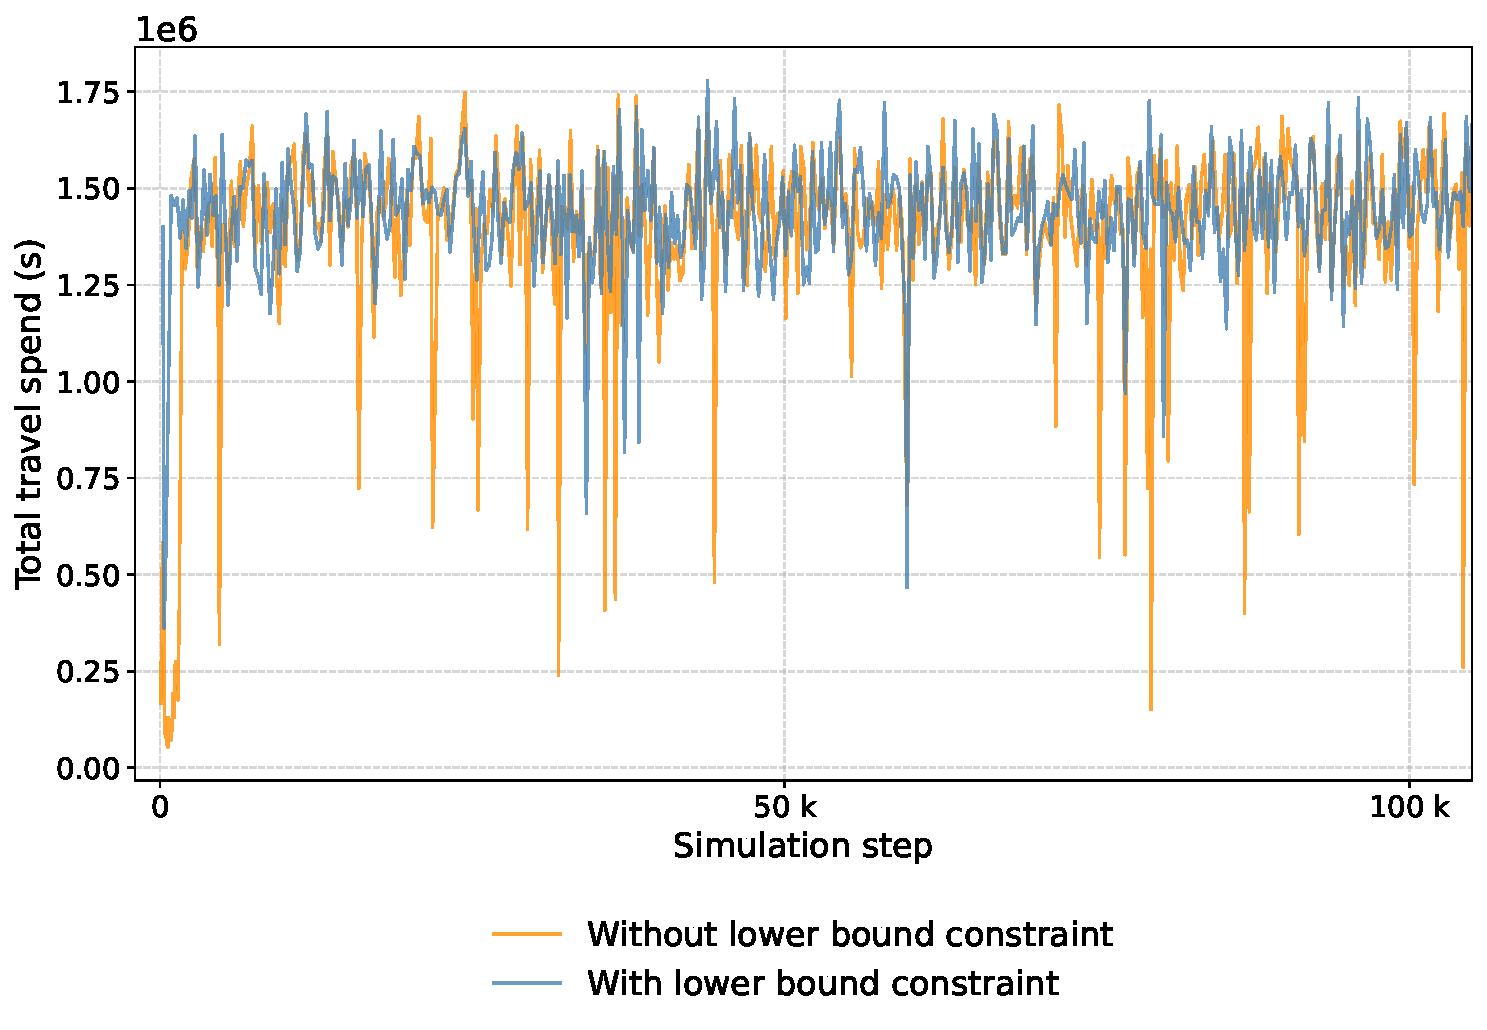
\includegraphics[width=0.95\linewidth]{figures/fig_9_rep.pdf}
        \caption{Cumulative TTS per training episode.}
        \label{fig:single_ramp_fig9_rep}
    \end{subfigure}
    \caption{Single-ramp training dynamics corresponding to Figures~8 and~9 of~\cite{Yang2025Reinforcement}. Orange denotes the baseline agent and blue the agent with action replacement.}
\end{figure*}

The original paper reports convergence at approximately $5 \times 10^4$ simulation steps. In the replication, both the episode length (Figure~\ref{fig:single_ramp_fig8_rep}) and TTS curves (Figure~\ref{fig:single_ramp_fig9_rep}) reach their steady-state mean rapidly (within $5 \times 10^3$ steps). The replacement curve (blue) continues to exhibit occasional severe drops later in the training process, most notably near $6 \times 10^4$ steps (see the episode length plot, Figure~\ref{fig:single_ramp_fig8_rep}). Despite this, it stabilises effectively after $8 \times 10^4$ steps. Across both metrics (Figures~\ref{fig:single_ramp_fig8_rep} and~\ref{fig:single_ramp_fig9_rep}), the constrained agent produces noticeably smoother curves with fewer and less severe early-termination events compared to the baseline agent (orange), which continues to fail periodically throughout the entire $1.2 \times 10^5$-step horizon. This dynamic directionally supports the paper's main claim that the action replacement module stabilises training by preventing ramp queue overflow, representing a successful structural replication of the original findings.

\paragraph{Figure 10 Replication.} Figure~\ref{fig:single_ramp_fig10_rep} shows the percentage of control steps at which the agent's action was overridden by the lower bound during each training episode.

The original paper reports a progressive reduction in the replacement percentage from approximately 23\% to nearly zero, which the authors interpret as the agent learning to proactively avoid unsafe states. In the replication, however, this metric decreases initially but stabilises at approximately 7\%, contradicting the original claim of near-zero convergence. This residual baseline may plausibly stem from two structural factors, though we did not isolate their individual contributions. First, entropy regularisation in the PPO objective ($c_e = 0.01$) discourages the policy's standard deviation from collapsing to zero, so stochastic action sampling could keep pushing some actions below the dynamic lower bound even after convergence. Second, the state representation lacks explicit temporal features, so the reactive policy may struggle to anticipate the lower bound's step change when demand shifts at $t = 600$\,s, potentially clustering replacements at that transition. We flag these as candidate explanations rather than confirmed mechanisms; distinguishing between them would require an ablation (e.g. varying $c_e$, or testing various constant and shifting demands).

\begin{figure}[!h]
    \centering
    \begin{subfigure}[b]{0.48\linewidth}
        \centering
        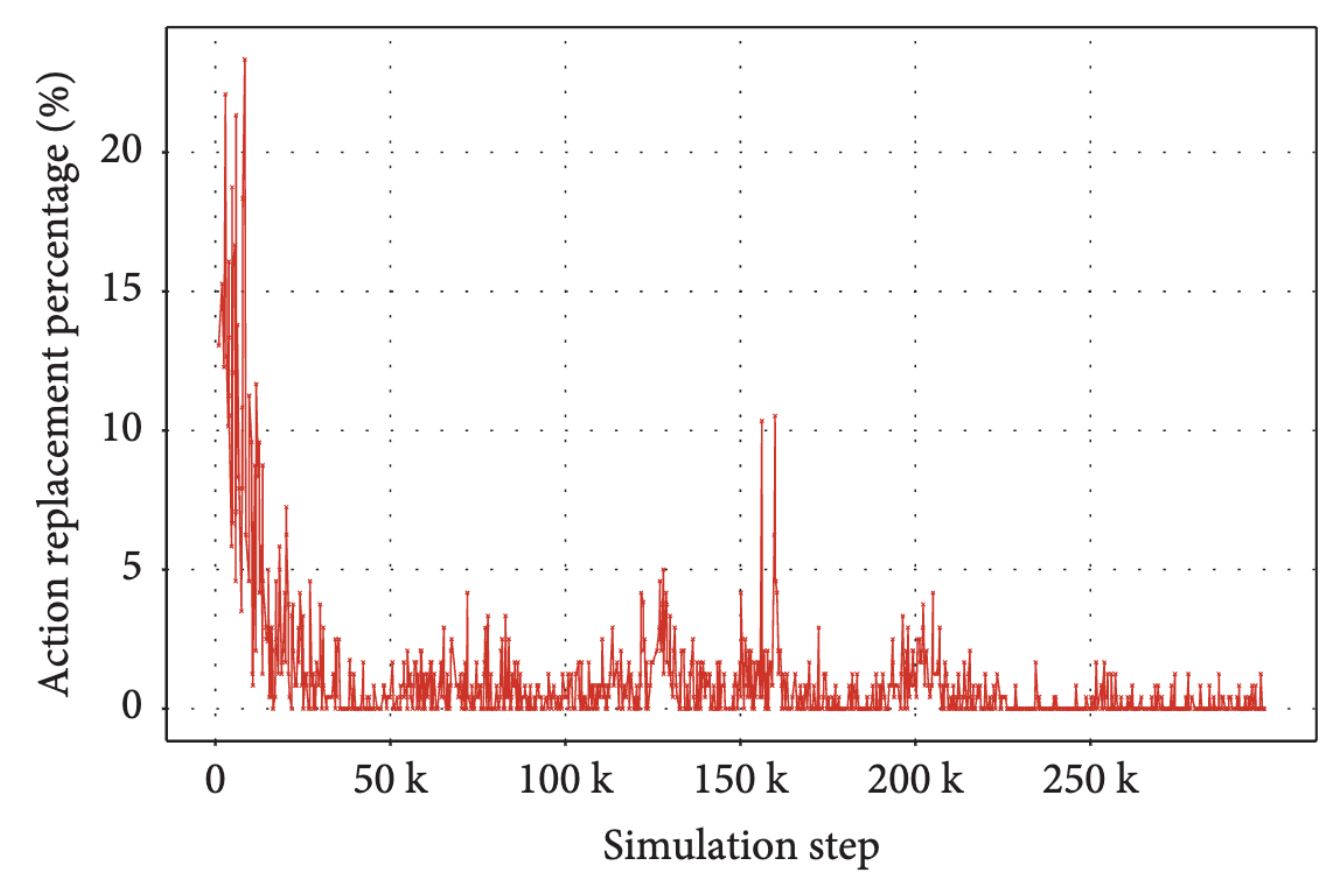
\includegraphics[width=\linewidth]{figures/yang2025_fig10.png}
        \caption{Original study}
        % \label{fig:fig6_orig}
    \end{subfigure}
    \hfill
    \begin{subfigure}[b]{0.48\linewidth}
        \centering
        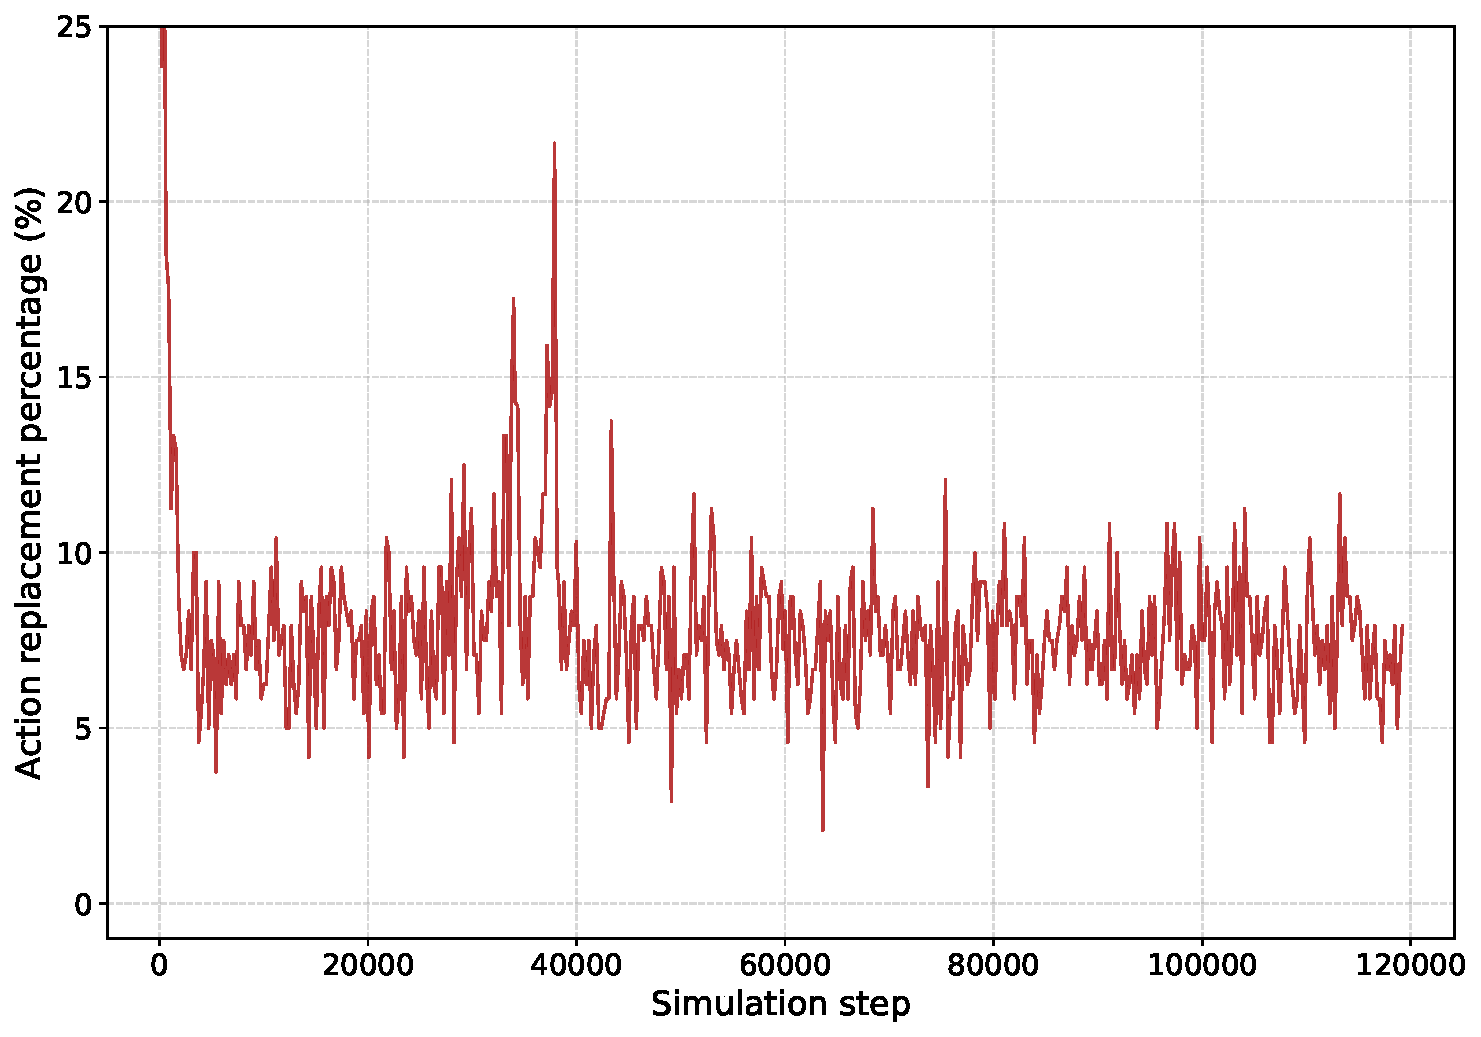
\includegraphics[width=\linewidth]{figures/fig_10_rep.pdf}
        \caption{Replicated study}
        % \label{fig:fig6_rep}
    \end{subfigure}
    \caption{Percentage of actions replaced by the lower bound constraint per episode during training (Demand~A), corresponding to Figure~10 of~\cite{Yang2025Reinforcement}. The original paper reports a decrease from $\approx25\%$ to $\approx0\%$; in the replication the replacement percentage decreases initially but stabilises at $\approx7\%$ for the remainder of training.}
    \label{fig:single_ramp_fig10_rep}
\end{figure}

\subsection{Multi-Ramp Scenario}

\subsubsection{Network and Environment Properties}

As detailed in Appendix~\ref{sec:assumptions}, the ramp capacities measured in the reconstructed SUMO network (1{,}900, 1{,}850, 1{,}850, and 1{,}950~veh$\cdot$h for ramps~1--4) are substantially below the paper-reported values (2{,}540, 2{,}650, 1{,}930, and 2{,}300~veh$\cdot$h). In the action replacement module the lower bound is computed using the paper-reported capacity values, consistent with the original formulation. Because the actual SUMO capacities are lower, the lower bound is calibrated to a throughput level the network cannot sustain, reducing how often the constraint is triggered in practice.

The original paper's Figure~13, which shows modified cumulative arrival curves for each of the four ramps demonstrating capacity drops at each downstream bottleneck, could not be reproduced. Generating the modified curves requires knowledge of the reference free-flow speed $q_0$ used to subtract the uniform-flow component, which is not reported in the original study and cannot be reliably inferred from the reconstructed network.


\subsubsection{Controller Performance -- Experiment~1}

Table~\ref{tab:multi_ramp_tts} compares the paper-reported values with the replication. The original study reports that PI-ALINEA, HERO, and RL all reduce TTS, with RL performing best. The replication also finds reductions for these three strategies, but with substantially different magnitudes.

\begin{table*}[t]
\centering
\caption{Multi-ramp cumulative TTS (veh$\cdot$h), percentage reduction relative to NC, and adjacent-network delay (veh$\cdot$h). Paper values are from Table~3 of~\cite{Yang2025Reinforcement}; replication values are means $\pm$ standard deviations over ten seeds. Replicated adjacent delay is approximated by time spent waiting to enter the simulation and is not directly comparable with the original metric.}
\label{tab:multi_ramp_tts}
\begin{tabular}{lrrrcrrc}
\toprule
& \multicolumn{3}{c}{\textbf{Original paper}} & & \multicolumn{3}{c}{\textbf{Replication}} \\
\cmidrule{2-4} \cmidrule{6-8}
\textbf{Strategy} & \textbf{TTS} & \textbf{Red.~(\%)} & \textbf{Delay} & & \textbf{TTS} & \textbf{Red.~(\%)} & \textbf{Delay} \\
\midrule
NC                   & 1901.43 & --       & 20.35   & & 1807.61 $\pm$ 48.52  & --          & 767.3 $\pm$ 40.5   \\
PI-ALINEA            & 1838.03 & 3.33     & 283.56  & & 1584.28 $\pm$ 28.61  & 12.35       & 871.3 $\pm$ 80.7   \\
HERO                 & 1756.70 & 7.61     & 447.69  & & 1587.23 $\pm$ 30.66  & 12.19       & 891.0 $\pm$ 64.6   \\
RL                   & 1630.45 & 14.25    & 354.52  & & 1341.58 $\pm$ 10.39  & 25.78       & 4076.1 $\pm$ 52.8   \\
RL \& Replacement    & --      & --       & 354.52  & & 1813.78 $\pm$ 30.11  & -0.34       & 747.8 $\pm$ 47.2   \\
\bottomrule
\end{tabular}
\end{table*}

The original adjacent-delay metric is not defined precisely. The replication uses cumulative waiting time before network insertion as a proxy, so these values are only qualitatively comparable.

The lower measured ramp capacities make active metering highly effective at protecting the mainline. PI-ALINEA and HERO produce similar TTS reductions of approximately 12\%. The unconstrained RL controller obtains the lowest mainline TTS, but its adjacent delay rises to $4{,}076.1$~veh$\cdot$h. The action distributions in Appendix~\ref{sec:appendix_results}, Figure~\ref{fig:action_distributions}, show why: the unconstrained agent selects metering rates near zero and effectively blocks the ramps, whereas the action replacement agent is forced toward rates near one to avoid queue spillback. The latter obtains a TTS slightly worse than NC, with a reduction of $-0.34\%$.

Figure~\ref{fig:multi_ramp_fig15_rep} in Appendix~\ref{sec:appendix_results} compares the space--time speed patterns. The NC scenario reproduces the approximate congestion formation and propagation. PI-ALINEA and HERO remove much more congestion than in the original study and are visually similar. The unconstrained RL controller almost eliminates mainline congestion, but only by transferring the delay upstream of the simulated network.

The training dynamics of the Experiment~1 agent are shown in Figure~\ref{fig:multi_ramp_fig14_rep}, which plots the episode TTS and cumulative episode reward over the training horizon, corresponding to Figure~14 of the original paper. The TTS (blue, left axis) decreases from approximately $4.3 \times 10^6$~s in the first episodes to a steady-state mean of approximately $3.9 \times 10^6$~s, while the episode reward (red, right axis) rises from approximately 80 to approximately 105. Both metrics stabilise within $5 \times 10^4$ simulation steps, consistent with the convergence point reported in the original paper. The original paper's Figure~14 shows the same dual-axis convergence pattern over the same approximate horizon, confirming that the Experiment~1 RL agent in the replication converges to a similarly efficient policy within a comparable training budget.

\begin{figure}[!h]
    \centering
    \begin{subfigure}[b]{0.48\linewidth}
        \centering
        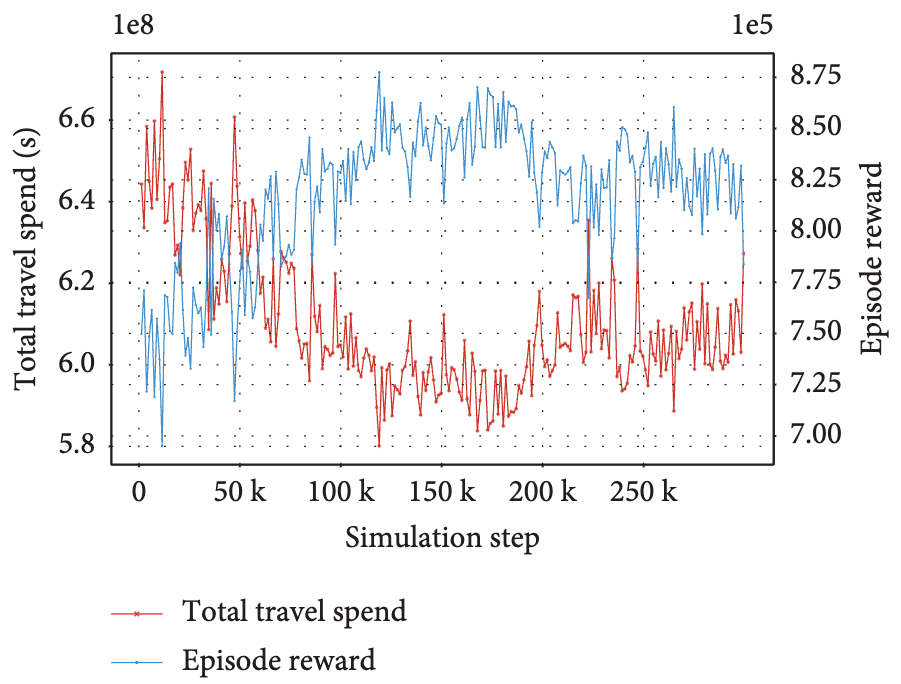
\includegraphics[width=\linewidth]{figures/yang2025_fig14.png}
        \caption{Original study}
    \end{subfigure}
    \hfill
    \begin{subfigure}[b]{0.48\linewidth}
        \centering
        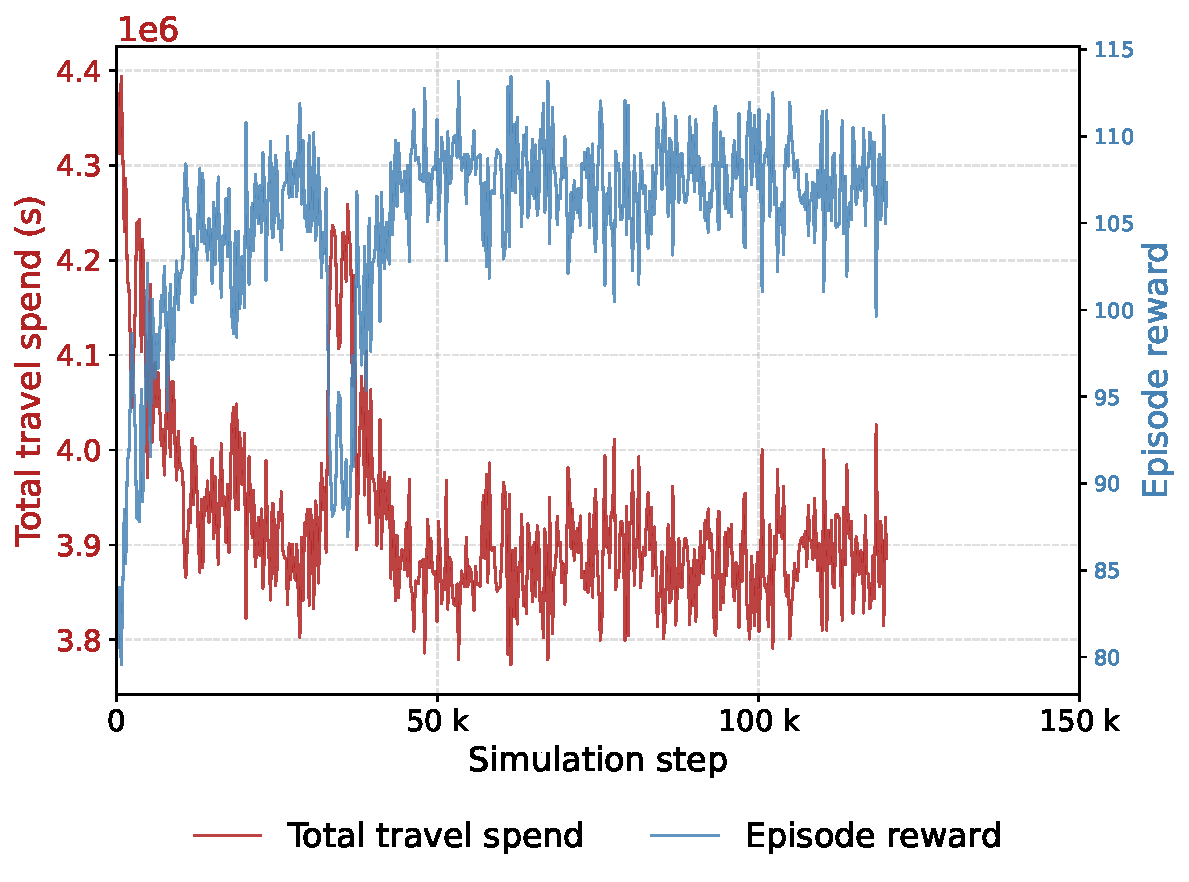
\includegraphics[width=\linewidth]{figures/fig_14_rep.pdf}
        \caption{Replicated study}
    \end{subfigure}
    \caption{Variation of episode TTS and cumulative episode reward during Experiment~1 training in the multi-ramp scenario, corresponding to Figure~14 of~\cite{Yang2025Reinforcement}. Top: original. Bottom: replication. TTS (blue, left axis) decreases from $\approx 4.3 \times 10^6$~s to a steady-state mean of $\approx 3.9 \times 10^6$~s; episode reward (red, right axis) rises from $\approx 80$ to $\approx 105$. Both metrics stabilise within $5 \times 10^4$ simulation steps.}
    \label{fig:multi_ramp_fig14_rep}
\end{figure}


\subsubsection{Training Dynamics and Action Replacement -- Experiment~2}
\label{sec:multi_ramp_training}

Experiment~2 differs from Experiment~1 in one critical respect: the ramp queue constraint is now strictly enforced during training. Whereas Experiment~1 imposed no hard limit on ramp queue length and relied entirely on the queue-spillback penalty term in the reward function to discourage overflow, Experiment~2 terminates any episode in which the queue length at any ramp exceeds $0.9 \cdot w_{\max}$. Spillback events therefore become directly observable as early-termination drops in the episode-length trajectory. Under this setup, two agents are trained and compared: a baseline agent that operates solely under the hard termination constraint but without the action replacement module (orange), and an agent equipped with the full action replacement module that additionally overrides unsafe actions with the store-and-forward lower bound $a_\mathrm{lb}$ and penalises them accordingly (blue). Because the enforced constraint prevents the agents from ever reaching the policy that caused the large adjacent-network delay seen in Experiment~1, both agents converge to a different, more conservative policy, as the original paper also notes.

Figures~\ref{fig:multi_ramp_fig16_rep} and~\ref{fig:multi_ramp_fig17_rep} show the episode lengths and cumulative TTS per episode over the first $1.5 \times 10^5$ simulation steps of Experiment~2 training.

\begin{figure*}[!h]
    \centering
    \begin{subfigure}[t]{0.49\linewidth}
        \centering
        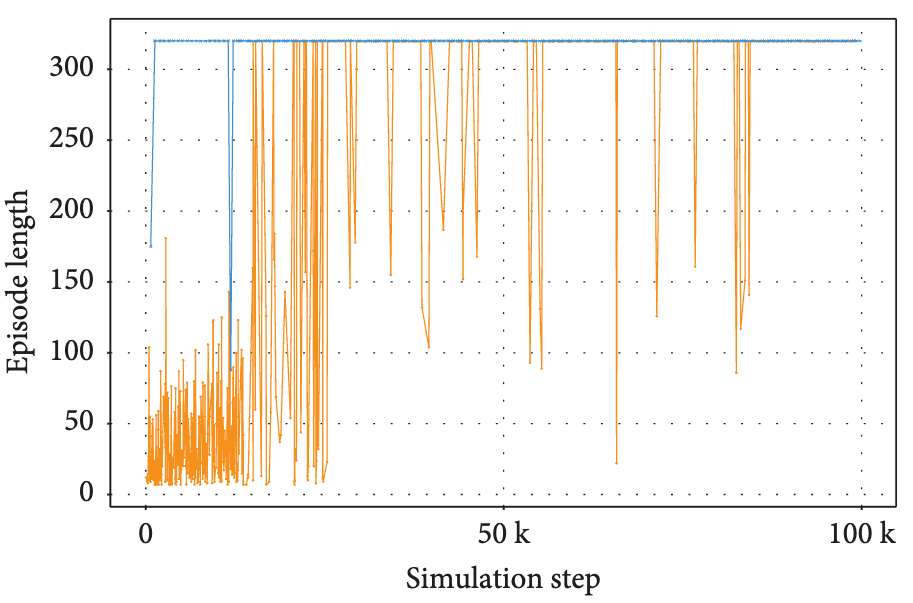
\includegraphics[width=0.9\linewidth]{figures/yang2025_fig16.png}
        \subcaption*{Original}
        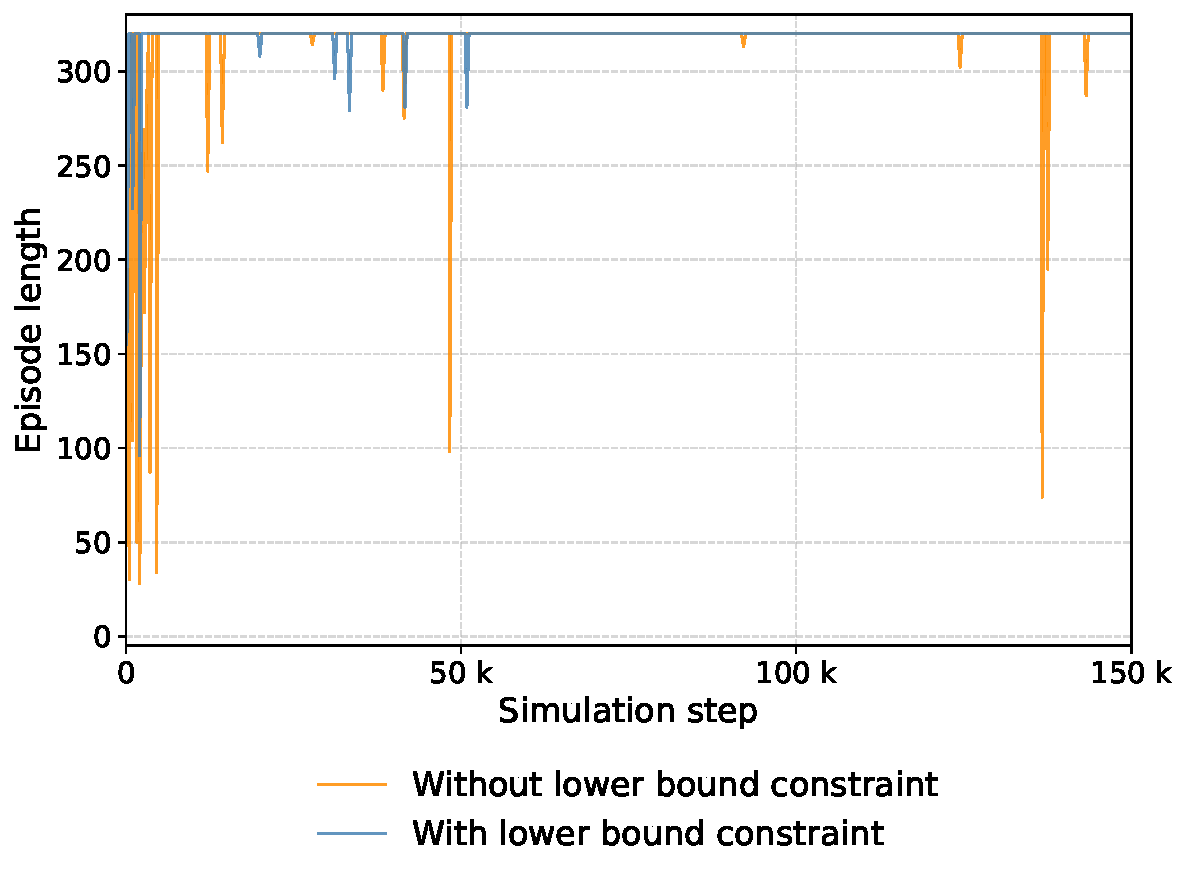
\includegraphics[width=0.9\linewidth]{figures/fig_16_rep.pdf}
        \subcaption*{Replication}
        \caption{Episode length. Drops below 320 steps indicate spillback termination.}
        \label{fig:multi_ramp_fig16_rep}
    \end{subfigure}
    \hfill
    \begin{subfigure}[t]{0.49\linewidth}
        \centering
        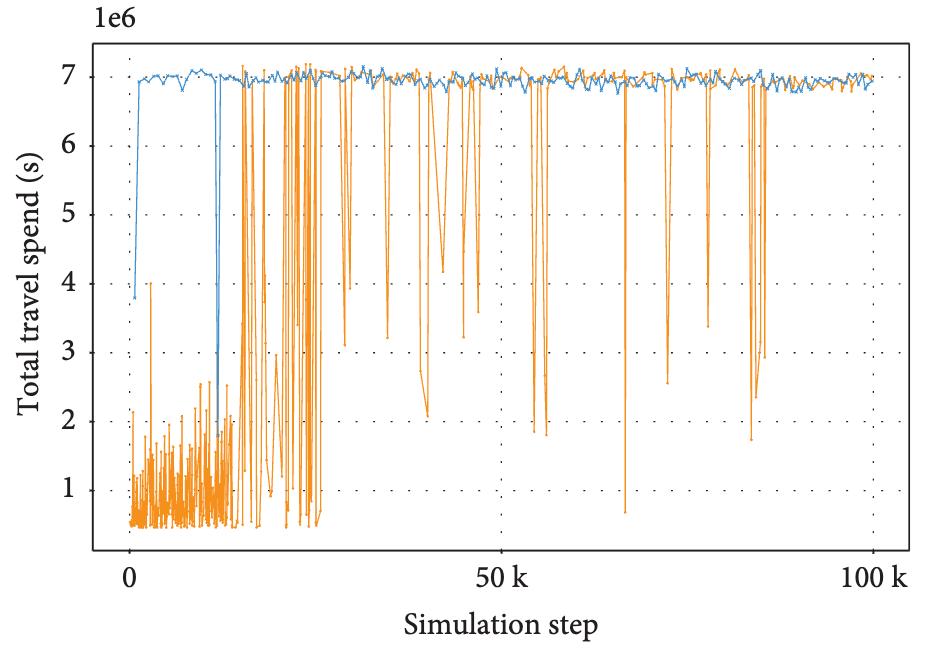
\includegraphics[width=0.9\linewidth]{figures/yang2025_fig17.png}
        \subcaption*{Original}
        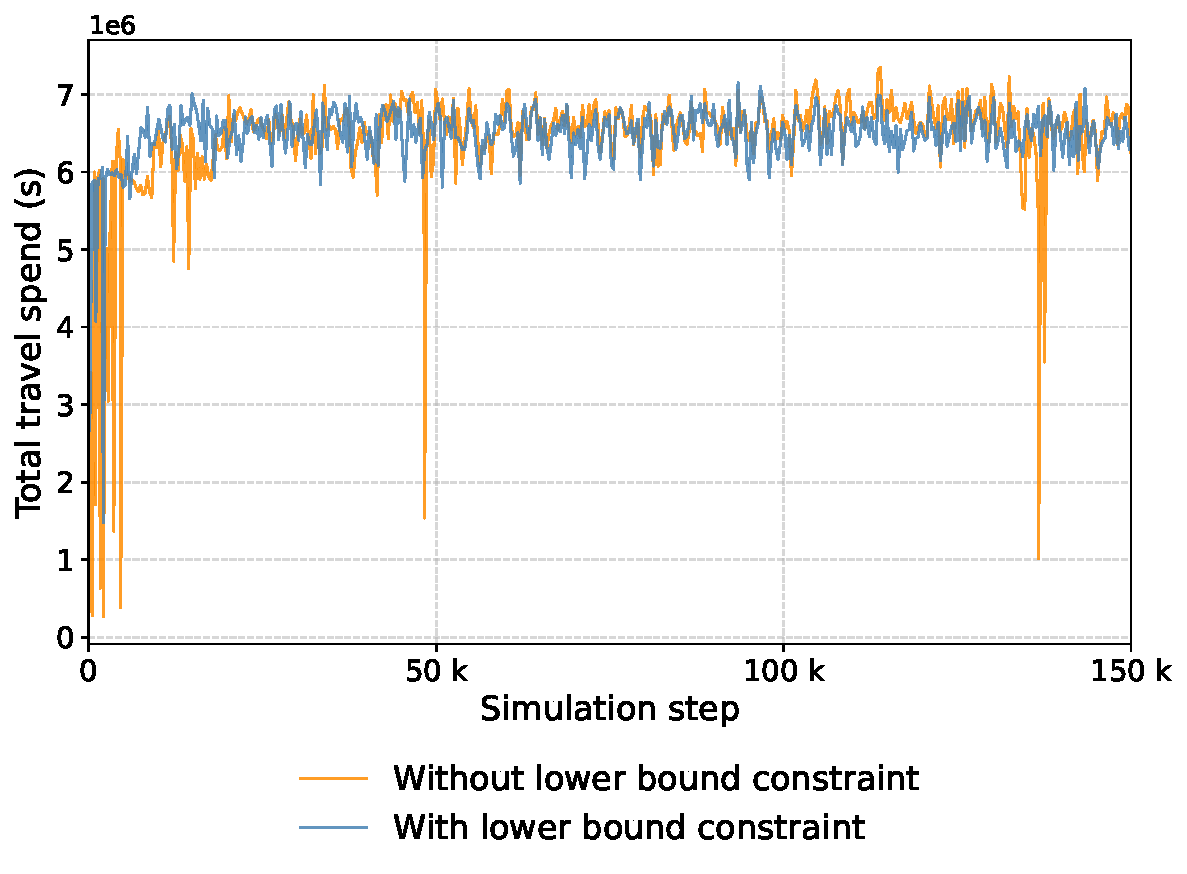
\includegraphics[width=0.9\linewidth]{figures/fig_17_rep.pdf}
        \subcaption*{Replication}
        \caption{Network TTS per training episode.}
        \label{fig:multi_ramp_fig17_rep}
    \end{subfigure}
    \caption{Multi-ramp Experiment~2 training dynamics corresponding to Figures~16 and~17 of~\cite{Yang2025Reinforcement}. Orange denotes the baseline and blue the agent with action replacement.}
\end{figure*}

Both agents suffer frequent early terminations during the first $\approx 10{,}000$ simulation steps, visible as sharp drops in Figure~\ref{fig:multi_ramp_fig16_rep} and as near-zero TTS spikes in Figure~\ref{fig:multi_ramp_fig17_rep}. After this initial exploration phase, both curves stabilise rapidly. The constrained agent (blue) reaches near-perfect episode completion—consistently achieving the maximum 320 control steps—within approximately $10^4$ steps and maintains this throughout the remainder of training, with only negligible exceptions. The unconstrained baseline (orange) similarly stabilises but retains two severe crash events at approximately $5 \times 10^4$ and $1.35 \times 10^5$ steps, where the episode length drops to as few as 100 and 80 steps respectively. These late-training spillback events indicate that the baseline policy, despite having largely converged, continues to discover unsafe action sequences that the lower bound constraint in the constrained agent permanently prevents. This pattern is consistent with the original paper's Figures~16 and~17, which show the constrained agent's episode length curve as notably smoother than the unconstrained baseline.

Within Experiment~2, the two agents converge to essentially identical steady-state TTS values of approximately $6.5 \times 10^6$~s (Figure~\ref{fig:multi_ramp_fig17_rep}). The action replacement module therefore improves training safety without degrading performance relative to the constrained baseline. This comparison does not imply that queue safety is cost-free relative to Experiment~1. The unconstrained Experiment~1 agent achieves a much lower mainline TTS by blocking the ramps and transferring delay upstream, whereas the Experiment~2 constraint prevents that unsafe policy.

Figure~\ref{fig:multi_ramp_fig18_rep} shows the proportion of control steps at which the agent's action was overridden by the lower bound during each training episode.

\begin{figure}[!h]
    \centering
    \begin{subfigure}[b]{0.48\linewidth}
        \centering
        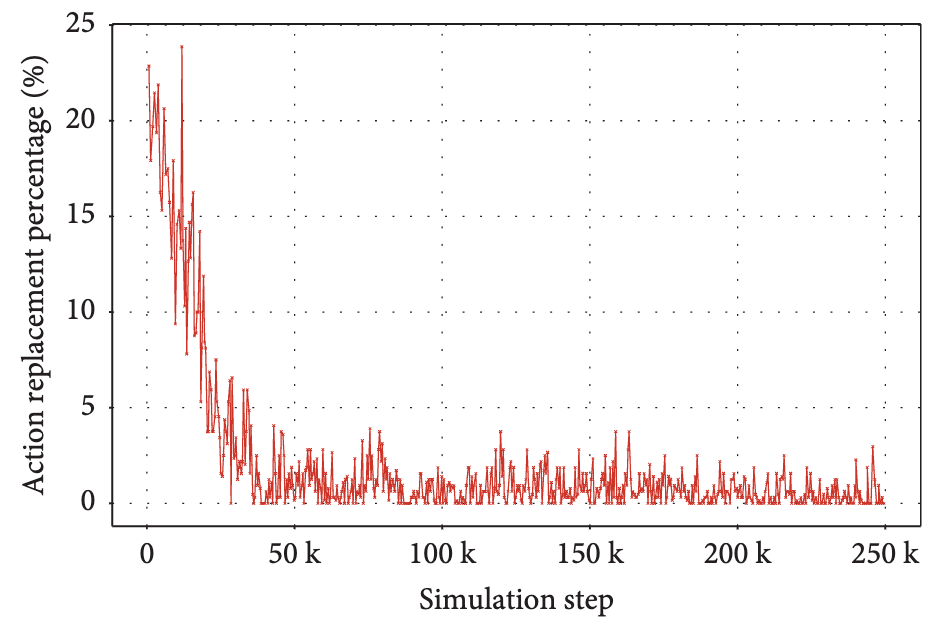
\includegraphics[width=\linewidth]{figures/yang2025_fig18.png}
        \caption{Original study}
    \end{subfigure}
    \hfill
    \begin{subfigure}[b]{0.48\linewidth}
        \centering
        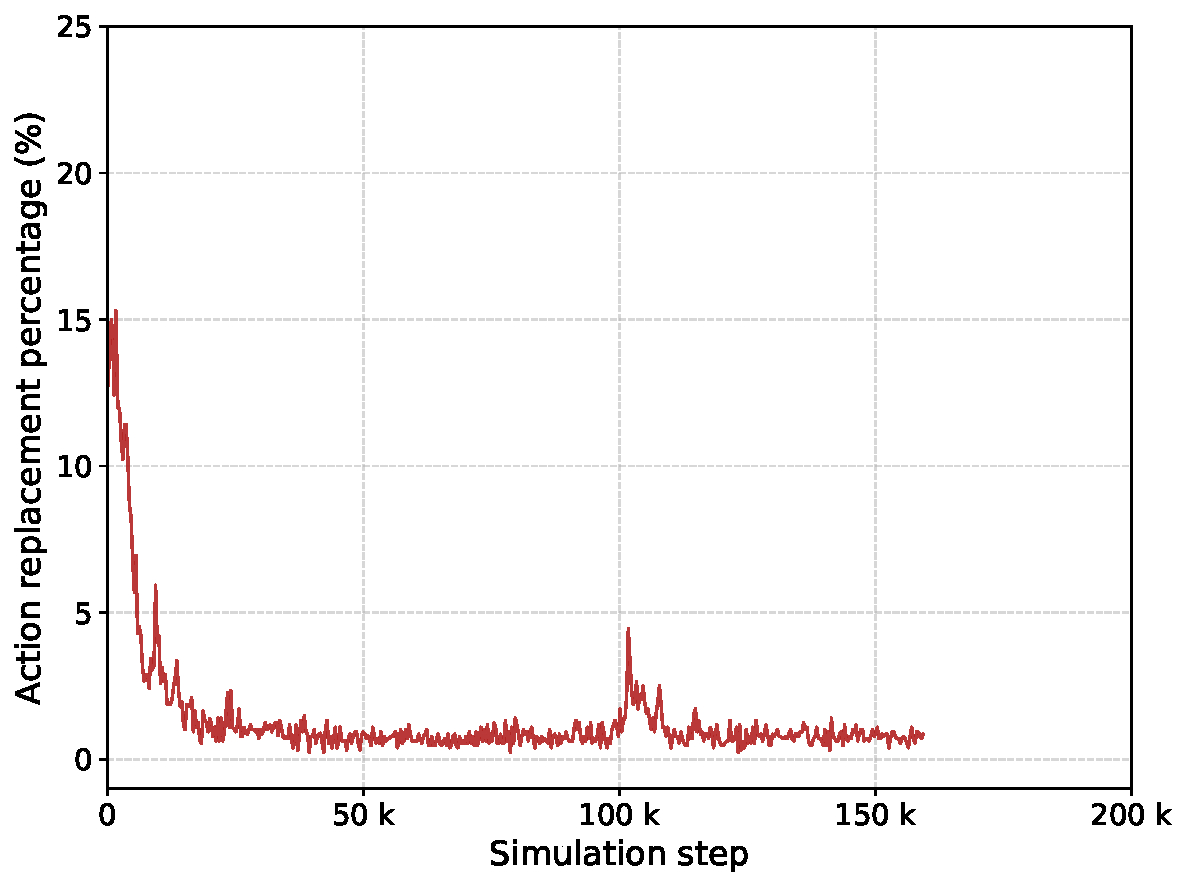
\includegraphics[width=\linewidth]{figures/fig_18_rep.pdf}
        \caption{Replicated study}
    \end{subfigure}
    \caption{Percentage of actions replaced by the lower bound constraint per episode during Experiment~2 training in the multi-ramp scenario, corresponding to Figure~18 of~\cite{Yang2025Reinforcement}. The original paper reports a decrease from $\approx 22.86\%$ to less than $1\%$; in the replication the replacement percentage decreases from $\approx 15\%$ to $\approx 1\%$ or below, with a transient spike to $\approx 4.5\%$ near $10^5$ steps coinciding with one of the unconstrained agent's crash events.}
    \label{fig:multi_ramp_fig18_rep}
\end{figure}

The replacement percentage begins at approximately $15\%$ in the first episodes, falls sharply to below $5\%$ within $5{,}000$ steps, and continues to decrease monotonically to approximately $1\%$ by $5 \times 10^4$ steps. A brief transient spike to $\approx 4.5\%$ occurs near $10^5$ steps before the curve returns to its converged level of approximately $0.5$--$1\%$. The original paper reports an initial replacement rate of $22.86\%$ decreasing to less than $1\%$ by the end of training. The replication reproduces this convergence to below $1\%$, providing the strongest quantitative agreement with the original paper of any figure in this replication study. As in the original, this trajectory is interpreted as evidence that the agent does not passively rely on the replacement mechanism indefinitely, but instead actively learns to issue metering rates that respect the store-and-forward lower bound.

This behaviour stands in contrast to the single-ramp scenario (Section~\ref{sec:single_ramp_training}), where the replacement percentage stabilised at approximately $7\%$ rather than converging to near zero. Several factors may contribute to this difference. One candidate is the initialisation of the actor log-standard-deviation, which differed between the two experiments. A higher initial log-standard-deviation in the single-ramp setup would produce wider action distributions throughout training, increasing the probability of stochastically sampling actions below the lower bound even after the policy mean has moved to a safe region. In the multi-ramp case, the constant demand profile also keeps the store-and-forward lower bound near its minimum value $a_{\min}$ for most of the episode, meaning that only extreme actions would trigger a replacement once the agent has learned a broadly safe policy. Under the stepwise demand used in the single-ramp scenario, the lower bound rises abruptly at the demand step at $t = 600$~s, creating transient windows where the already-converged policy is temporarily out of safe range. These environmental differences, together with any hyperparameter variation, likely all contribute to the different residual replacement rates, and disentangling their individual contributions would require a dedicated ablation study.

Overall, the multi-ramp Experiment~2 results represent the strongest replication outcome. Episode stability, TTS convergence within Experiment~2, and the declining replacement percentage are reproduced, and the final replacement rate of approximately 1\% agrees quantitatively with the original paper. The safety claim is therefore directionally verified, but the reconstructed congested network exposes a trade-off between protecting ramp queues and minimising mainline TTS.

\subsection{Critical Remarks}

The replication produced a mixed result. The multi-ramp Experiment~2 safety behaviour was reproduced most closely: action replacement reduced late spillback failures, did not degrade performance relative to the constrained baseline, and declined to approximately 1\% of actions. The single-ramp experiment also showed smoother training, but the replacement rate stabilised near 7\%. The reported TTS reductions and several traffic patterns were not reproduced.

The original study does not follow several experimental practices needed to evaluate reinforcement-learning methods reliably. It does not report the number of random seeds, uncertainty estimates, or TTS performance for the proposed safe controller. Its training figures show single trajectories without variance bands. Important network parameters, demand profiles, hyperparameters, and implementation details are also omitted. These omissions prevent a direct reconstruction of the experiments and make it difficult to separate the effect of the proposed method from the effect of the simulation configuration.

Despite these limitations, the underlying proposal is interesting. The action replacement module explicitly tracks the remaining storage capacity of each ramp and uses this information to constrain unsafe actions during training. This provides a practical connection between physical queue limits and reinforcement-learning control. Our results indicate that the mechanism can improve training safety. However, stronger evidence requires evaluation across multiple seeds, clearly specified demand regimes, and openly available simulation environments and code.

The most critical missing details required to accurately reproduce the paper's results include:

\begin{itemize}
    \item SUMO network parameters and geometry details, including max speed limits, distance between the ramp exit and ramp traffic light, and exact lane configurations and connection types at the merge zones and downstream mainline.
    \item The explicit definition and measurement methodology for mainline and ramp capacities.
    \item The maximum queue storage capacity ($w_{max}$) for each ramp in the multi-ramp scenario.
    \item The state representation and dimensionality used in the multi-ramp scenario.
    \item TTS performance values for the proposed safe RL controller with the action replacement module.
    \item Full mainline and ramp demand time-series profiles for the multi-ramp scenario, including how flow leaving through the four off-ramps was accounted for.
\end{itemize}


\section{Conclusion}
\label{sec:conclusion}

We independently replicated the safe reinforcement-learning ramp-metering method proposed by Yang et al.~\cite{Yang2025Reinforcement}. The SUMO networks, demand profiles, controllers, and training pipeline were reconstructed from the published article because the original implementation and simulation files were unavailable.

The results support the qualitative value of the action replacement module but do not reproduce the original study's quantitative performance claims. The strongest agreement was obtained in the multi-ramp safety experiment: action replacement reduced spillback failures, preserved performance relative to the constrained baseline, and declined to approximately 1\% of actions. The single-ramp experiment showed a weaker safety benefit, and its replacement rate remained near 7\%. Absolute TTS reductions and several reported traffic patterns differed substantially from the original results.

These differences are closely tied to missing demand data, network parameters, training settings, and metric definitions. The action replacement concept is therefore promising, but its reported performance cannot be independently verified from the article alone. Releasing complete simulation networks, executable code, exact demand profiles, and results across multiple random seeds is necessary for a conclusive evaluation of the method.









